
%%%%%%%%%%%%%%%%%%%%%%%%%%%%%%%%%%%%%%%%%%%%%%%%%%%%%%%%
%
% Copyright (c) 2003-2009 by University of Queensland
% Earth Systems Science Computational Center (ESSCC)
% http://www.uq.edu.au/esscc
%
% Primary Business: Queensland, Australia
% Licensed under the Open Software License version 3.0
% http://www.opensource.org/licenses/osl-3.0.php
%
%%%%%%%%%%%%%%%%%%%%%%%%%%%%%%%%%%%%%%%%%%%%%%%%%%%%%%%%

\documentclass{manual}

% grab the handy definitions and \usepackage statements etc

%%%%%%%%%%%%%%%%%%%%%%%%%%%%%%%%%%%%%%%%%%%%%%%%%%%%%%%%%%%%%%%%%%%%%%%%%%%%%%
% Copyright (c) 2003-2017 by The University of Queensland
% http://www.uq.edu.au
%
% Primary Business: Queensland, Australia
% Licensed under the Apache License, version 2.0
% http://www.apache.org/licenses/LICENSE-2.0
%
% Development until 2012 by Earth Systems Science Computational Center (ESSCC)
% Development 2012-2013 by School of Earth Sciences
% Development from 2014 by Centre for Geoscience Computing (GeoComp)
%
%%%%%%%%%%%%%%%%%%%%%%%%%%%%%%%%%%%%%%%%%%%%%%%%%%%%%%%%%%%%%%%%%%%%%%%%%%%%%%

\usepackage{subfigure}
\usepackage{epsfig}

\usepackage{graphicx,color}
% \usepackage[pdftex]{graphicx,color}
\usepackage{makeidx}  % handle the index properly
\usepackage{xspace}   % handle spaces after commands more nicely
% use the ams math stuff, as it makes the maths easier to code, and
% nicer output than the standard LaTeX stuff
\usepackage{amsmath,amsfonts,amssymb} % this is handy for mathematicians and physici % see http://www.ams.org/tex/amslatex.html
\usepackage{alltt}   % handy verbatim stuff
\usepackage{textcomp}
\usepackage{setspace}
%\usepackage{movie15}
% Special Formatting Packages
% Colour Package
\usepackage[usenames,dvipsnames]{xcolor}
% Assignm Colour Names and import hyperlinks.
\usepackage{float}
%\usepackage[unicode,colorlinks=true,linkcolor=NavyBlue,citecolor=OliveGreen,urlcolor=Plum]{hyperref}

% Fancy Verb


\usepackage[numbers]{natbib}
\usepackage{chapterbib}
\renewcommand{\bibname}{References}

%\doublespacing

%% Python listing setup
% from http://blog.miliauskas.lt/2008/09/python-syntax-highlighting-in-latex.html

\usepackage{color}
\usepackage[procnames]{listings}
\usepackage{textcomp}
\usepackage{setspace}
\usepackage{palatino}
\renewcommand{\lstlistlistingname}{Code Listings}
\renewcommand{\lstlistingname}{Code Listing}
\definecolor{gray}{gray}{0.5}
\definecolor{green}{rgb}{0,0.5,0}
\definecolor{lightgreen}{rgb}{0,0.7,0}
\definecolor{purple}{rgb}{0.5,0,0.5}
\definecolor{darkred}{rgb}{0.5,0,0}
\definecolor{orange}{rgb}{1.0,0.4,0.1}
\lstnewenvironment{python}[1][]{
\lstset{
language=python,
basicstyle=\ttfamily\small\setstretch{1},
stringstyle=\color{green},
showstringspaces=false,
alsoletter={1234567890},
otherkeywords={\ , \}, \{},
keywordstyle=\color{blue},
emph={access,and,as,break,class,continue,def,del,elif,else,%
except,exec,finally,for,from,global,if,import,in,is,%
lambda,not,or,pass,print,raise,return,try,while,assert},
emphstyle=\color{orange}\bfseries,
emph={[2]self},
emphstyle=[2]\color{gray},
emph={[4]ArithmeticError,AssertionError,AttributeError,BaseException,%
DeprecationWarning,EOFError,Ellipsis,EnvironmentError,Exception,%
False,FloatingPointError,FutureWarning,GeneratorExit,IOError,%
ImportError,ImportWarning,IndentationError,IndexError,KeyError,%
KeyboardInterrupt,LookupError,MemoryError,NameError,None,%
NotImplemented,NotImplementedError,OSError,OverflowError,%
PendingDeprecationWarning,ReferenceError,RuntimeError,RuntimeWarning,%
StandardError,StopIteration,SyntaxError,SyntaxWarning,SystemError,%
SystemExit,TabError,True,TypeError,UnboundLocalError,UnicodeDecodeError,%
UnicodeEncodeError,UnicodeError,UnicodeTranslateError,UnicodeWarning,%
UserWarning,ValueError,Warning,ZeroDivisionError,abs,all,any,apply,%
basestring,bool,buffer,callable,chr,classmethod,cmp,coerce,compile,%
complex,copyright,credits,delattr,dict,dir,divmod,enumerate,eval,%
execfile,exit,file,filter,float,frozenset,getattr,globals,hasattr,%
hash,help,hex,id,input,int,intern,isinstance,issubclass,iter,len,%
license,list,locals,long,map,max,min,object,oct,open,ord,pow,property,%
quit,range,raw_input,reduce,reload,repr,reversed,round,set,setattr,%
slice,sorted,staticmethod,str,sum,super,tuple,type,unichr,unicode,%
vars,xrange,zip},
emphstyle=[4]\color{purple}\bfseries,
upquote=true,
morecomment=[s][\color{lightgreen}]{"""}{"""},
commentstyle=\color{red}\slshape,
literate={>>>}{\textbf{\textcolor{darkred}{>{>}>}}}3%
         {...}{{\textcolor{gray}{...}}}3,
procnamekeys={def,class},
procnamestyle=\color{blue}\textbf,
%framexleftmargin=1mm, framextopmargin=1mm, frame=box,
%rulesepcolor=\color{gray},#1
}}{}



%%%%%%%%%%%%%%%%%%%%%%%%%%%%%%%%%%%%%%%%%%%%%%%%%%%%%%%%%%%%%%%%%%%%%%%%%%%%%%
% Copyright (c) 2003-2015 by University of Queensland
% http://www.uq.edu.au
%
% Primary Business: Queensland, Australia
% Licensed under the Open Software License version 3.0
% http://www.opensource.org/licenses/osl-3.0.php
%
% Development until 2012 by Earth Systems Science Computational Center (ESSCC)
% Development 2012-2013 by School of Earth Sciences
% Development from 2014 by Centre for Geoscience Computing (GeoComp)
%
%%%%%%%%%%%%%%%%%%%%%%%%%%%%%%%%%%%%%%%%%%%%%%%%%%%%%%%%%%%%%%%%%%%%%%%%%%%%%%

\usepackage{listing}
% defines the colour for the background of code examples
\definecolor{LightGrey}{gray}{0.9}

%Some colour definitions added to keep pdflatex happy
%I make no claim that these values are particularly good
\definecolor{Purple}{rgb}{0.7, 0, 0.6}
\definecolor{Tan}{rgb}{0.5,0.5,0.5}
\definecolor{BrickRed}{rgb}{0.7, 0.2, 0.2}
\definecolor{Black}{rgb}{0, 0, 0}

% All the \color{x} used to be \color[named]{x}
%end color defs

\lstdefinestyle{myC++}{%
language=C++,
showstringspaces=false,
basicstyle=\small\ttfamily,
commentstyle=\color{BrickRed}\ttfamily,
keywordstyle=\color{Purple}\ttfamily,
%identifierstyle=\color{Blue}\ttfamily,
%functionstyle=\color{Blue}\ttfamily,
%typestyle=\color{ForestGreen}\ttfamily,
stringstyle=\color{Tan}\ttfamily,%
morekeywords={,complex,}%
frame=none,%
backgroundcolor=\color{LightGrey}%
}

\lstdefinestyle{myMatlab}{%
language=Matlab,
showstringspaces=false,
basicstyle=\small\ttfamily,
commentstyle=\color{BrickRed}\ttfamily,
keywordstyle=\color{Purple}\ttfamily,
%identifierstyle=\color{Blue}\ttfamily,
%functionstyle=\color{Blue}\ttfamily,
%typestyle=\color{ForestGreen}\ttfamily,
stringstyle=\color{Tan}\ttfamily,%
frame=none,%
backgroundcolor=\color{LightGrey}%
}

\lstdefinestyle{myScilab}{%
language=Scilab,
showstringspaces=false,
basicstyle=\small\ttfamily,
commentstyle=\color{BrickRed}\ttfamily,
keywordstyle=\color{Purple}\ttfamily,
%identifierstyle=\color{Blue}\ttfamily,
%functionstyle=\color{Blue}\ttfamily,
%typestyle=\color{ForestGreen}\ttfamily,
stringstyle=\color{Tan}\ttfamily,%
frame=none,%
backgroundcolor=\color{LightGrey}%
}

\lstdefinestyle{myShell}{%
language=ksh,
showstringspaces=false,
basicstyle=\small\ttfamily,
commentstyle=\color{Black}\ttfamily,
keywordstyle=\color{Black}\ttfamily,
%identifierstyle=\color{Blue}\ttfamily,
%functionstyle=\color{Blue}\ttfamily,
%typestyle=\color{ForestGreen}\ttfamily,
stringstyle=\color{Black}\ttfamily,%
frame=none,%
backgroundcolor=\color{LightGrey}%
}

\lstdefinestyle{myPython}{%
language=python,
showstringspaces=false,
basicstyle=\small\ttfamily,
commentstyle=\color{BrickRed}\ttfamily,
keywordstyle=\color{Purple}\ttfamily,
%identifierstyle=\color{Blue}\ttfamily,
%functionstyle=\color{Blue}\ttfamily,
%typestyle=\color{ForestGreen}\ttfamily,
stringstyle=\color{Tan}\ttfamily,%
frame=none,%
%backgroundcolor=\color{LightGrey}%
}

\lstdefinestyle{myhtml}{%
language=xml,
showstringspaces=false,
basicstyle=\small\ttfamily,
commentstyle=\color{BrickRed}\ttfamily,
keywordstyle=\color{Purple}\ttfamily,
%identifierstyle=\color{Blue}\ttfamily,
%functionstyle=\color{Blue}\ttfamily,
%typestyle=\color{ForestGreen}\ttfamily,
stringstyle=\color{Tan}\ttfamily,
morekeywords={,simulation,prop_dim,error_check,stochastic,%
  globals,field,dimensions,lattice,domains,samples,vector,%
  components,fourier_space,sequence,integrate,algorithm,%
  interval,k_operators,constant,operator_names,vectors,%
  output,filename,group,sampling,moments,benchmark,use_double,%
  use_wisdom,use_prefs,binary_output,cycles,filter,post_propagation,%
  default_value,argv,arg,iterations,cross_propagation,%
  use_mpi,paths,seed,noises,author,description,name,type,%
}
frame=none,%
%framerule=2pt,%
backgroundcolor=\color{LightGrey}%
}


% this implements producing nice code blocks
% it also saves time, typing and
% *should* reduce errors in the text by removing doubling up of code
\lstnewenvironment{xmdsCode}[1][]{\lstset{style=myhtml}\lstset{#1}}{}

% this implements nicely formatted shell code
\lstnewenvironment{shellCode}[1][]{\lstset{style=myShell}\lstset{#1}}{}

% this implements nicely formatted Perl code
\lstnewenvironment{perlCode}[1][]{\lstset{style=myPerl}\lstset{#1}}{}

% this implements nicely formatted Python code
\lstnewenvironment{python}[1][]{\lstset{style=myPython}\lstset{#1}}{}

% this implements nicely formatted C++ code
\lstnewenvironment{CCode}{\lstset{style=myC++}}{}

% this implements nicely formatted matlab code
\lstnewenvironment{matlabCode}{\lstset{style=myMatlab}}{}

% this implements nicely formatted scilab code
\lstnewenvironment{scilabCode}{\lstset{style=myScilab}}{}



%Ensures that latex doesn't have an error if we don't specify the version
\providecommand{\RepVersion}{Unknown\xspace}

%Tony's Commands
\newcommand{\editor}[1] {\textit{EDITORIAL: {#1}}}
\newcommand{\fileex}[1]{\module{examples\textbackslash {#1}}\xspace}
\newcommand{\TODO}[1]{\textbf{TODO}:\xspace\textit{#1} } 
\newcommand{\TBA}[1]{\textbf{TO BE ADDED: \begin{enumerate} {#1} \end{enumerate}}}
%\newcommand{\eqref}[1] {(\ref{#1})}

% text names
\newcommand{\esys}{\textit{esys}\xspace}
\newcommand{\pyt}{\textit{python}\xspace}
\newcommand{\esc}{\textit{escript}\xspace}
\newcommand{\FINLEY}{\textit{finley}\xspace}
\newcommand{\ripley}{\textit{ripley}\xspace}
\newcommand{\speckley}{\textit{speckley}\xspace}
\newcommand{\exf}{\textit{doc/examples/cookbook/}\xspace}
\newcommand{\mayavi}{\textit{Mayavi2}\xspace}

%referencing
\newcommand{\reffig}[1]{Figure~(\ref{#1})}
\newcommand{\refeq}[1]{equation~(\ref{#1})}
\newcommand{\refEq}[1]{Equation~(\ref{#1})}
\newcommand{\refCh}[1]{Chapter~\ref{#1}}
\newcommand{\refSec}[1]{Section~\ref{#1}}


%modules
\newcommand{\modesys}{\module{esys}\xspace}
\newcommand{\modescript}{\module{esys.escript}\xspace}
\newcommand{\modLPDE}{\module{esys.escript.LinearPDEs}\xspace}
\newcommand{\modfinley}{\module{esys.finley}\xspace}
\newcommand{\modpycad}{\module{esys.pycad}\xspace}
\newcommand{\modvtk}{\module{vtk}\xspace}
\newcommand{\modnumpy}{\module{numpy}\xspace}
\newcommand{\modmpl}{\module{matplotlib}\xspace}
\newcommand{\pycad}{\module{esys.pycad}\xspace}
\newcommand{\gmsh}{\module{esys.pycad.gmsh}\xspace}
\newcommand{\pylab}{\module{pylab}\xspace}
\newcommand{\mpl}{\module{matplotlib}\xspace}
\newcommand{\numpy}{\module{numpy}\xspace}
\newcommand{\weipa}{\module{esys.weipa}\xspace}

%list scripts
\newcommand{\sslist}[1]{\textbf{The scripts referenced in this section are; #1} \newline \newline}


% title, author, etc stuff
\title{The Escript COOKBOOK}

\ifpdf
\pdfinfo {
/Author (Antony Hallam)
/Title (escript COOKBOOK)
/Keywords (escript, PDEs)
}
\fi

\author{Antony Hallam}
\authoraddress{
Earth Systems Science Computational Centre (ESSCC) \\
School of Earth Sciences \\
The University of Queensland \\
Brisbane, Australia \\
Email: \email{esys@esscc.uq.edu.au}
}                                                                                         
\date{\today}      
\release{Alpha}
\setshortversion{}

\makeindex

\begin{document}

\maketitle

\tableofcontents

\chapter{Introduction}
%%%%%%%%%%%%%%%%%%%%%%%%%%%%%%%%%%%%%%%%%%%%%%%%%%%%%%%%
%
% Copyright (c) 2003-2012 by University of Queensland
% Earth Systems Science Computational Center (ESSCC)
% http://www.uq.edu.au/esscc
%
% Primary Business: Queensland, Australia
% Licensed under the Open Software License version 3.0
% http://www.opensource.org/licenses/osl-3.0.php
%
%%%%%%%%%%%%%%%%%%%%%%%%%%%%%%%%%%%%%%%%%%%%%%%%%%%%%%%%

\chapter{Introduction}
This document describes how to install \emph{esys-Escript}\footnote{For the rest of the document we will drop the \emph{esys-}} on your computer.
To learn how to use \esfinley please see the Cookbook, User's guide or the API documentation.
If you use the Debian or Ubuntu packages to install then the documentation will be available in
\file{/usr/share/doc/escript}, otherwise (if you haven't done so already) you can download the documentation bundle 
from launchpad.

\esfinley is primarily developed on Linux desktop, SGI ICE and \macosx systems.
It is distributed in two forms:
\begin{enumerate}
  \item Binary bundles -- these are great for first time users or for those who want to start using 
    \esfinley immediately.
      Bundles are available for:
      \begin{itemize}
	  \item Debian and Ubuntu Linux distributions ($32$/$64$-bit i686) (.deb package)
	  \item Linux desktop systems with gcc (stand-alone bundle)
	  \item \macosx Leopard systems (also tested on Lion) with gcc (stand-alone bundle)
	  \item $32$bit Windows (requires some other packages to be installed).
      \end{itemize}    
    Please see Chapter~\ref{chap:bin} for instructions on how to install the binary bundles \esfinley.
  \item Source bundles -- these require compilation and should be used if the binary bundles 
    don't work on the target machine or if extra functionality is required such as \mpi parallelisation.
    See Chapter~\ref{chap:compiler} for detailed instructions.
\end{enumerate}

See the site \url{https://answers.launchpad.net/escript-finley} for online help.

\section{Significant changes since version 3.3}
\begin{itemize}
 \item \texttt{SymPy} is now required to compile or run \escript. 
    This means you will need to download sympy in addition to the support bundle from previous releases.
 \item The minimum Python version is now $2.6$.
\end{itemize}

% \noindent If you choose to compile from source your options are to
% \begin{itemize}
%     \item install dependencies (e.g. using your package manager) and only compile \esfinley, OR
%     \item compile everything from source.
% \end{itemize}
% Either way, please see Chapter~\ref{chap:compiler} for a discussion of compiler features.
% Compiling \esfinley when its dependencies are already installed is discussed in Chapter~\ref{chap:essrc}.
% To compile \esfinley and all dependencies from source please see Chapter~\ref{chap:allsrc}.
% The latter option takes a significant amount of time and is only required if the versions of the dependent libraries available on your system do not work with \esfinley.
% 
% Once everything is installed you can test your installation using the Python scripts in \file{examples.zip} or \file{examples.tar.gz}\footnote{These should either be in \file{escript.d/release/doc} or in the case of Debian, in \file{/usr/share/doc/escript}.}.
% Unpack the examples and try to run the following from a terminal:
% \begin{shellCode}
%  run-escript poission.py
% \end{shellCode}
% If this produces a VTK file called \file{u.vtu} then you are likely to have a functional \esfinley installation.
% You can try and visualize the VTK data or delete the file.
% For visualization we suggest using \file{VisIt}\footnote{\url{https://wci.llnl.gov/codes/visit/}} or \file{MayaVi}\footnote{\url{http://mayavi.sourceforge.net}} which are both freely available.







%%%%%%%%%%%%%%%%%%%%%%%%%%%%%%%%%%%%%%%%%%%%%%%%%%%%%%%%
%
% Copyright (c) 2003-2009 by University of Queensland
% Earth Systems Science Computational Center (ESSCC)
% http://www.uq.edu.au/esscc
%
% Primary Business: Queensland, Australia
% Licensed under the Open Software License version 3.0
% http://www.opensource.org/licenses/osl-3.0.php
%
%%%%%%%%%%%%%%%%%%%%%%%%%%%%%%%%%%%%%%%%%%%%%%%%%%%%%%%%

\section{Quickstart}
For information on how to install and run \esc please look at the installation and users guides which are available for download from launchpad at  \url{https://launchpad.net/escript-finley/+download}.

%%%%%%%%%%%%%%%%%%%%%%%%%%%%%%%%%%%%%%%%%%%%%%%%%%%%%%%%%%%%%%%%%%%%%%%%%%%%%%
% Copyright (c) 2003-2016 by The University of Queensland
% http://www.uq.edu.au
%
% Primary Business: Queensland, Australia
% Licensed under the Apache License, version 2.0
% http://www.apache.org/licenses/LICENSE-2.0
%
% Development until 2012 by Earth Systems Science Computational Center (ESSCC)
% Development 2012-2013 by School of Earth Sciences
% Development from 2014 by Centre for Geoscience Computing (GeoComp)
%
%%%%%%%%%%%%%%%%%%%%%%%%%%%%%%%%%%%%%%%%%%%%%%%%%%%%%%%%%%%%%%%%%%%%%%%%%%%%%%

\section{Escript and Python Basics} \label{sec:escpybas}

The \pyt scripting language is a powerful and easy to learn environment with a wide variety of applications. \esc has been developed as a packaged module for \pyt specifically to solve complex partial differential equations. As a result, all the conventions and programming syntax associated with \pyt are coherent with \esc. If you are unfamiliar with \pyt, there are a large number of simple to advanced guides and tutorials available online. These texts should provide an introduction that is comprehensive enough to use \esc. A handful of \pyt tutorials are listed below.
\begin{itemize}
\item \url{http://hetland.org/writing/instant-python.html} is a very crisp introduction. It covers everything you need to get started with \esc.
\item A nice and easy to follow introduction: \url{http://www.sthurlow.com/python/}
\item Another crisp tutorial: \url{http://www.zetcode.com/tutorials/pythontutorial/}. 
 \item A very comprehensive tutorial from the \pyt authors: \url{http://www.python.org/doc/2.5.2/tut/tut.html}. It covers much more than what you will ever need for \esc.
\item Another comprehensive tutorial: \url{http://www.tutorialspoint.com/python/index.htm}
\end{itemize} 

\subsection{The \modesys Modules}
\esc is part of the \esys package. 
Apart from the particle simulation library
\verb|ESyS-Particle|\footnote{see \url{https://launchpad.net/esys-particle}} which is not covered
in this tutorial \esys also includes the following modules
\begin{enumerate}
\item \modescript is the PDE solving module.
\item \modfinley is the discretisation tool and finite element package.
\item \modpycad  is a package for creating irregular shaped domains.
\end{enumerate}
Further explanations of each of these are available in the \esc user guide or in the API documentation\footnote{Available from \url{https://launchpad.net/escript-finley/+download}}. 
\esc is also dependent on a few other open-source packages which are not maintained by the \esc development team. These are \modnumpy (an array and matrix handling package), \modmpl \footnote{\modnumpy and \modmpl are part of the SciPy package, see \url{http://www.scipy.org/}} (a simple plotting tool) and \verb gmsh \footnote{See \url{http://www.geuz.org/gmsh/}} (which is required by \modpycad). These packages (\textbf{except} for \verb gmsh ) are included with the support bundles. 



%%%%%%%%%%%%%%%%%%%%%%%%%%%%%%%%%%%%%%%%%%%%%%%%%%%%%%%%%%%%%%%%%%%%%%%%%%%%%%
% Copyright (c) 2003-2012 by University of Queensland
% http://www.uq.edu.au
%
% Primary Business: Queensland, Australia
% Licensed under the Open Software License version 3.0
% http://www.opensource.org/licenses/osl-3.0.php
%
% Development until 2012 by Earth Systems Science Computational Center (ESSCC)
% Development since 2012 by School of Earth Sciences
%
%%%%%%%%%%%%%%%%%%%%%%%%%%%%%%%%%%%%%%%%%%%%%%%%%%%%%%%%%%%%%%%%%%%%%%%%%%%%%%

\chapter{The Einstein Summation Convention}

The Einstein Summation Convention (ESC) is a notational convention that is prefered by the \esc developers. It is a condensed and practical way to deal with multi-dimensional and convoluted PDEs. By suppressing the need to write out the many terms of each problem it is possible to increase efficiency and reduce the number of errors created through poor working. According to the convention, when an index variable appears twice in a single term, it implies that we are summing over all of its possible values.
So we have;
\begin{equation}
a_{1}\frac{\partial^2 f}{\partial x_{1}^2} + a_{2}\frac{\partial^2 f}{\partial x_{2}^2} = a_{i}\frac{\partial^2 f}{\partial x_{i}^2}
\end{equation}

For a scalar function $f(x_{1},x_{2},..x_{i})$ and a vector $\mathbf{u}(u_{1},u_{2},..u_{i})$ with $u_{i}(x_{1},x_{2},..x_{i})$, we have the following notation:
\begin{equation}
\mathbf{u}=\sum_{i}u_{i}e^i = u_{i}e^i
\end{equation}
\begin{equation}
\mathbf{grad}(f) = \mathbf{\nabla}(f) = \sum_{i}\frac{\partial f}{\partial x_{i}}e^i = (\partial_{i} f)e^i = f_{,i}e^i
\end{equation}
\begin{equation}
div(\mathbf{u}) = \mathbf{\nabla}.\mathbf{u} = \sum_{i}\frac{\partial u_{i}}{\partial x_{i}} = \partial_{i} u_{i} = u_{i,i}
\end{equation}
\begin{equation}
div(\mathbf{grad}(f)) = \nabla^2 f = \Delta f = \sum_{i}\frac{\partial^2 f}{\partial x_{i}^2} = f_{,ii}
\end{equation}


%%%%%%%%%%%%%%%%%%%%%%%%%%%%%%%%%%%%%%%%%%%%%%%%%%%%%%%%
%
% Copyright (c) 2003-2009 by University of Queensland
% Earth Systems Science Computational Center (ESSCC)
% http://www.uq.edu.au/esscc
%
% Primary Business: Queensland, Australia
% Licensed under the Open Software License version 3.0
% http://www.opensource.org/licenses/osl-3.0.php
%
%%%%%%%%%%%%%%%%%%%%%%%%%%%%%%%%%%%%%%%%%%%%%%%%%%%%%%%%

\section{An introduction to Partial Differential Equations}
Maybe not assuming enough prior knowledge from the reader here, this section may be redundant as a result.


\chapter{Getting Started with Heat Diffusion}

%%%%%%%%%%%%%%%%%%%%%%%%%%%%%%%%%%%%%%%%%%%%%%%%%%%%%%%%
%
% Copyright (c) 2003-2010 by University of Queensland
% Earth Systems Science Computational Center (ESSCC)
% http://www.uq.edu.au/esscc
%
% Primary Business: Queensland, Australia
% Licensed under the Open Software License version 3.0
% http://www.opensource.org/licenses/osl-3.0.php
%
%%%%%%%%%%%%%%%%%%%%%%%%%%%%%%%%%%%%%%%%%%%%%%%%%%%%%%%%

\begin{figure}[h!]
\centerline{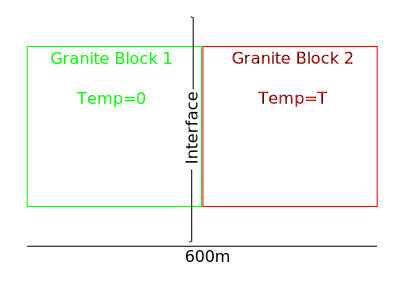
\includegraphics[width=4.in]{figures/onedheatdiff001}}
\caption{Temperature differential along a single interface between two granite blocks.}
\label{fig:onedgbmodel}
\end{figure}

\section{One Dimensional Heat Diffusion in Granite}
\label{Sec:1DHDv00}

The first model consists of two blocks of isotropic material, for instance granite, sitting next to each other.
Initially, \textit{Block 1} is of a temperature
\verb|T1| and \textit{Block 2} is at a temperature \verb|T2|.
We assume that the system is insulated.
What would happen to the temperature distribution in each block over time? 
Intuition tells us that heat will transported from the hotter block to the cooler until both
blocks have the same temperature.

\subsection{1D Heat Diffusion Equation}
We can model the heat distribution of this problem over time using the one dimensional heat diffusion equation\footnote{A detailed discussion on how the heat diffusion equation is derived can be found at \url{http://online.redwoods.edu/instruct/darnold/DEProj/sp02/AbeRichards/paper.pdf}};
which is defined as:
\begin{equation}
\rho c\hackscore p \frac{\partial T}{\partial t} - \kappa \frac{\partial^{2} T}{\partial x^{2}} = q\hackscore H 
\label{eqn:hd}
\end{equation}
where $\rho$ is the material density, $c\hackscore p$ is the specific heat and $\kappa$ is the thermal 
conductivity\footnote{A list of some common thermal conductivities is available from Wikipedia \url{http://en.wikipedia.org/wiki/List_of_thermal_conductivities}}. Here we assume that these material 
parameters are \textbf{constant}. 
The heat source is defined by the right hand side of \refEq{eqn:hd} as $q\hackscore{H}$; this can take the form of a constant or a function of time and space. For example $q\hackscore{H} = q\hackscore{0}e^{-\gamma t}$ where we have the output of our heat source decaying with time. There are also two partial derivatives in \refEq{eqn:hd}; $\frac{\partial T}{\partial t}$ describes the change in temperature with time while $\frac{\partial ^2 T}{\partial x^2}$ is the spatial change of temperature. As there is only a single spatial dimension to our problem, our temperature solution $T$ is only dependent on the time $t$ and our position along the iron bar $x$.

\subsection{PDEs and the General Form}
Potentially, it is now possible to solve PDE \refEq{eqn:hd} analytically and this would produce an exact solution to our problem. However, it is not always possible or practical to solve a problem this way. Alternatively, computers can be used to solve these kinds of problems. To do this, a numerical approach is required to discretised 
the PDE \refEq{eqn:hd} in time and space so finally we are left with a finite number of equations for a finite number of spatial and time steps in the model. While discretization introduces approximations and a degree of error, we find that a sufficiently sampled model is generally accurate enough for the requirements of the modeller.

Firstly, we will discretise the PDE \refEq{eqn:hd} in the time direction which will
leave as with a steady linear PDE which is involving spatial derivatives only and needs to be solved in each time 
step to progress in time - \esc can help us here.

For the discretization in time we will use is the Backwards Euler approximation scheme\footnote{see \url{http://en.wikipedia.org/wiki/Euler_method}}. It bases on the
approximation 
\begin{equation}
\frac{\partial T(t)}{\partial t} \approx \frac{T(t)-T(t-h)}{h}
\label{eqn:beuler}
\end{equation}
for  $\frac{\partial T}{\partial t}$  at time $t$ 
where $h$ is the time step size. This can also be written as;
\begin{equation}
\frac{\partial T}{\partial t}(t^{(n)}) \approx \frac{T^{(n)} - T^{(n-1)}}{h}
\label{eqn:Tbeuler}
\end{equation}
where the upper index $n$ denotes the n\textsuperscript{th} time step. So one has
\begin{equation}
\begin{array}{rcl}
t^{(n)} & = & t^{(n-1)}+h \\
T^{(n)} & = & T(t^{(n-1)}) \\ 
\end{array}
\label{eqn:Neuler}
\end{equation}
Substituting \refEq{eqn:Tbeuler} into \refEq{eqn:hd} we get;
\begin{equation}
\frac{\rho c\hackscore p}{h} (T^{(n)} - T^{(n-1)}) - \kappa \frac{\partial^{2} T^{(n)}}{\partial x^{2}} = q\hackscore H 
\label{eqn:hddisc}
\end{equation}
Notice that we evaluate the spatial derivative term at current time $t^{(n)}$ - therefore the name \textbf{backward Euler} scheme. Alternatively, one can use evaluate the spatial derivative term at the previous time $t^{(n-1)}$. This 
approach is called the \textbf{forward Euler} scheme. This scheme can provide some computational advantages which
we are not discussed here but has the major disadvantage that depending on the 
material parameter as well as the discretization of the spatial derivative term the time step size $h$ needs to be chosen sufficiently small to achieve a stable temperature when progressing in time. The term \textit{stable} means
that the approximation of the temperature will not grow beyond its initial bounds and becomes non-physical. 
The backward Euler which we use here is unconditionally stable meaning that under the assumption of
physically correct problem set-up the temperature approximation remains physical for all times. 
The user needs to keep in mind that the discretization error introduced by \refEq{eqn:beuler} 
is sufficiently small so a good approximation of the true temperature is calculated. It is
therefore crucial that the user remains critical about his/her results and for instance compares 
the results for different time and spatial step sizes. 

To get the temperature $T^{(n)}$ at time $t^{(n)}$ we need to solve the linear 
differential equation \refEq{eqn:hddisc} which is only including spatial derivatives. To solve this problem
we want to to use \esc. 

\esc interfaces with any given PDE via a general form. For the purpose of this introduction we will illustrate a simpler version of the full linear PDE general form which is available in the \esc user's guide. A simplified form that suits our heat diffusion problem\footnote{In the form of the \esc users guide which using the Einstein convention is written as 
$-(A\hackscore{jl} u\hackscore{,l})\hackscore{,j}+D u =Y$}
is described by;
\begin{equation}\label{eqn:commonform nabla}
-\nabla\cdot(A\cdot\nabla u) + Du = f
\end{equation}
where $A$, $D$ and $f$ are known values and $u$ is the unknown solution. The symbol $\nabla$ which is called the \textit{Nabla operator} or \textit{del operator} represents
the spatial derivative of its subject - in this case $u$. Lets assume for a moment that we deal with a one-dimensional problem then ;
\begin{equation}
\nabla = \frac{\partial}{\partial x}
\end{equation}
and we can write \refEq{eqn:commonform nabla} as;
\begin{equation}\label{eqn:commonform}
-A\frac{\partial^{2}u}{\partial x^{2}} + Du = f
\end{equation}
if $A$ is constant. To match this simplified general form to our problem \refEq{eqn:hddisc} 
we rearrange \refEq{eqn:hddisc};
\begin{equation}
\frac{\rho c\hackscore p}{h} T^{(n)} - \kappa \frac{\partial^2 T^{(n)}}{\partial x^2} = q\hackscore H +  \frac{\rho c\hackscore p}{h} T^{(n-1)}
\label{eqn:hdgenf}
\end{equation}
The PDE is now in a form that satisfies \refEq{eqn:commonform nabla} which is required for \esc to solve our PDE. This can be done by generating a solution for successive increments in the time nodes $t^{(n)}$ where 
$t^{(0)}=0$ and  $t^{(n)}=t^{(n-1)}+h$ where $h>0$ is the step size and assumed to be constant. 
In the following the upper index ${(n)}$ refers to a value at time $t^{(n)}$. Finally, by comparing \refEq{eqn:hdgenf} with \refEq{eqn:commonform} it can be seen that;
\begin{equation}\label{ESCRIPT SET}
u=T^{(n)}; 
A = \kappa; D = \frac{\rho c \hackscore{p}}{h}; f = q \hackscore{H} + \frac{\rho c\hackscore p}{h} T^{(n-1)}
\end{equation}

\subsection{Boundary Conditions}
\label{SEC BOUNDARY COND}
With the PDE sufficiently modified, consideration must now be given to the boundary conditions of our model. Typically there are two main types of boundary conditions known as \textbf{Neumann} and \textbf{Dirichlet} boundary conditions\footnote{More information on Boundary Conditions is available at Wikipedia \url{http://en.wikipedia.org/wiki/Boundary_conditions}}, respectively. 
A \textbf{Dirichlet boundary condition} is conceptually simpler and is used to prescribe a known value to the unknown - in our example the temperature - on parts of the boundary or on the entire boundary of the region of interest. 
We discuss Dirichlet boundary condition in our second example presented in Section~\ref{Sec:1DHDv0}.

We make the model assumption that the system is insulated so we need
to add an appropriate boundary condition to prevent
any loss or inflow of energy at boundary of our domain. Mathematically this is expressed by prescribing
the heat flux $\kappa \frac{\partial T}{\partial x}$  to zero. In our simplified one dimensional model this is expressed
in the form;
\begin{equation}
\kappa \frac{\partial T}{\partial x}  = 0 
\end{equation}
or in a more general case as
\begin{equation}\label{NEUMAN 1}
\kappa \nabla T \cdot n  = 0 
\end{equation}
where $n$  is the outer normal field \index{outer normal field} at the surface of the domain. 
The $\cdot$ (dot) refers to the  dot product of the vectors $\nabla T$ and $n$. In fact, the term $\nabla T \cdot n$ is the normal derivative of 
the temperature $T$. Other notations which are used are\footnote{The \esc notation for the normal
derivative is $T\hackscore{,i} n\hackscore i$.};
\begin{equation}
\nabla T \cdot n  = \frac{\partial T}{\partial n} \; .
\end{equation}
A condition of the type \refEq{NEUMAN 1} defines a \textbf{Neuman boundary condition} for the PDE. 

The PDE \refEq{eqn:hdgenf} 
and the Neuman boundary condition~\ref{eqn:hdgenf} (potentially together with the Dirichlet boundary condition set)  define a \textbf{boundary value problem}. 
It is a nature of a boundary value problem that it allows to make statements on the solution in the
interior of the domain from information known on the boundary only. In most cases
we use the term partial differential equation but in fact mean a boundary value problem. 
It is important to keep in mind that boundary conditions need to be complete and consistent in the sense that 
at any point on the boundary either a Dirichlet or a Neuman boundary condition must be set.

Conveniently, \esc makes default assumption on the boundary conditions which the user may modify where appropriate. 
For a problem of the form in~\refEq{eqn:commonform nabla} the default condition\footnote{In the form of the \esc users guide which is using the Einstein convention is written as 
$n\hackscore{j}A\hackscore{jl} u\hackscore{,l}=0$.} is;
\begin{equation}\label{NEUMAN 2}
n\cdot A \cdot\nabla u = 0 
\end{equation}
which is used everywhere on the boundary. Again $n$ denotes the outer normal field. 
Notice that the coefficient $A$ is the same as in the \esc PDE~\ref{eqn:commonform nabla}. 
With the settings for the coefficients we have already identified in \refEq{ESCRIPT SET} this
condition translates into 
\begin{equation}\label{NEUMAN 2b}
\kappa \frac{\partial T}{\partial x} = 0 
\end{equation}
for the boundary of the domain. This is identical to the Neuman boundary condition we want to set. \esc will take care of this condition for us. We will discuss the Dirichlet boundary condition later.

\subsection{Outline of the Implementation}
\label{sec:outline}
To solve the heat diffusion equation (equation \refEq{eqn:hd}) we will write a simple \pyt script. At this point we assume that you have some basic understanding of the \pyt programming language. If not there are some pointers and links available in Section \ref{sec:escpybas}. The script we will discuss later in details will have four major steps. Firstly we need to define the domain where we want to 
calculate the temperature. For our problem this is the joint blocks of granite which has a rectangular shape. Secondly we need to define the PDE 
we need to solve in each time step to get the updated temperature. Thirdly we need to define the the coefficients of the PDE and finally we need to solve the PDE. The last two steps need to be repeated until the final time marker has been reached. As a work flow this takes the form;
\begin{enumerate}
 \item create domain
 \item create PDE
 \item while end time not reached:
\begin{enumerate}
 \item set PDE coefficients
 \item solve PDE
 \item update time marker
\end{enumerate}
\item end of calculation
\end{enumerate}
In the terminology of \pyt the domain and PDE are represented by \textbf{objects}. The nice feature of an object is that it defined by it usage and features
rather than its actual representation. So we will create a domain object to describe the geometry of the two
granite blocks. The main feature 
of the object we will use is the fact that we can define PDEs and spatially distributed values such as the temperature 
on a domain. In fact the domain object has many more features - most of them you will 
never use and do not need to understand. Similar a PDE object is defined by the fact that we can define the coefficients of the PDE and solve the PDE. At a 
later stage you may use more advanced features of the PDE class but you need to worry about them only at the point when you use them.


\begin{figure}[t]
 \centering
   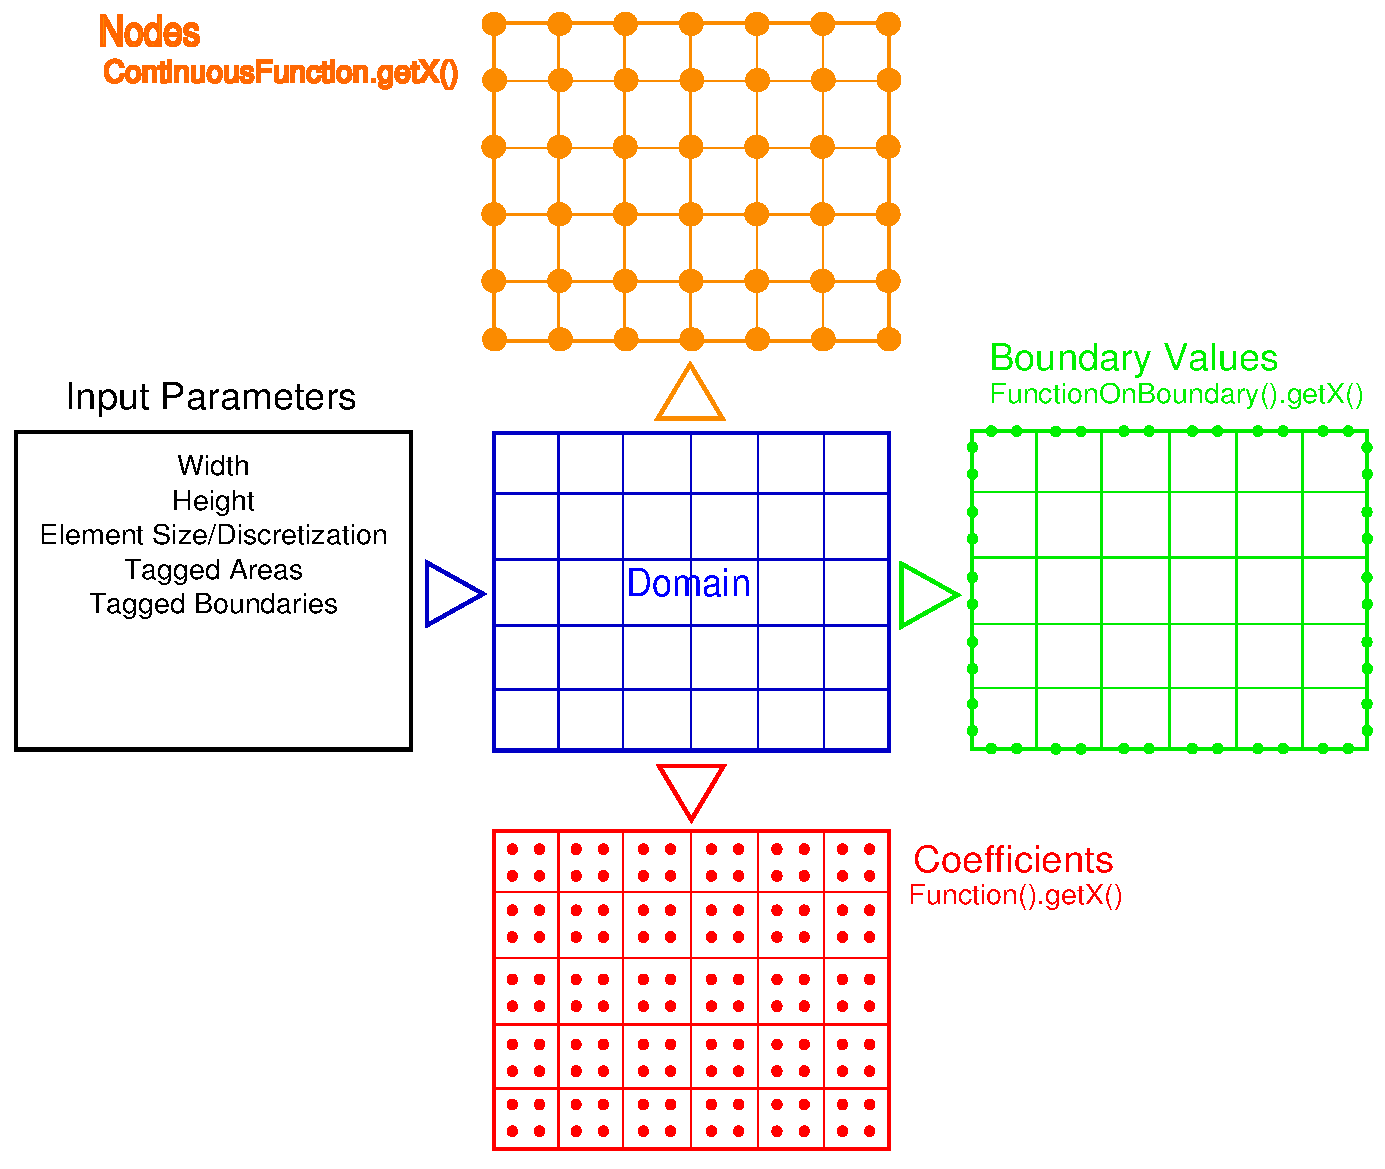
\includegraphics[width=6in]{figures/functionspace.pdf}
   \label{fig:fs}
   \caption{\esc domain construction overview}
\end{figure}

\subsection{The Domain Constructor in \esc}
\label{ss:domcon}
It is helpful to have a better understanding how spatially distributed value such as the temperature or PDE coefficients are interpreted in \esc. Again
from the user's point of view the representation of these spatially distributed values is not relevant. 

There are various ways to construct domain objects. The simplest form is as rectangular shaped region with a length and height. There is
a ready to use function call for this. Besides the spatial dimensions the function call will require you to specify the number
elements or cells to be used along the length and height, see \reffig{fig:fs}. Any spatially distributed value 
and the PDE is represented in discrete form using this element representation\footnote{We will use the finite element method (FEM), see \url{http://en.wikipedia.org/wiki/Finite_element_method} for details.}. Therefore we will have access to an approximation of the true PDE solution only. 
The quality of the approximation depends - besides other factors- mainly on the number of elements being used. In fact, the 
approximation becomes better the more elements are used. However, computational costs and compute time grow with the number of
elements being used. It therefore important that you find the right balance between the demand in accuracy and acceptable resource usage.

In general, one can thinks about a domain object as a composition of nodes and elements. 
As shown in \reffig{fig:fs}, an element is defined by the nodes used to describe its vertices. 
To represent spatial distributed values the user can use 
the values at the nodes, at the elements in the interior of the domain or at elements located at the surface of the domain. 
The different approach used to represent values is called \textbf{function space} and is attached to all objects
in \esc representing a spatial distributed value such as the solution of a PDE. The three 
function spaces we will use at the moment are;
\begin{enumerate}
\item the nodes, called by \verb|ContinuousFunction(domain)| ;
\item the elements/cells, called by \verb|Function(domain)| ; and
\item the boundary, called by \verb|FunctionOnBoundary(domain)| .
\end{enumerate}
A function space object such as \verb|ContinuousFunction(domain)| has the method \verb|getX| attached to it. This method returns the
location of the so-called \textbf{sample points} used to represent values with the particular function space attached to it. So the
call \verb|ContinuousFunction(domain).getX()| will return the coordinates of the nodes used to describe the domain while
the  \verb|Function(domain).getX()| returns the coordinates of numerical integration points within elements, see
\reffig{fig:fs}. 

This distinction between different representations of spatial distributed values 
is important in order to be able to vary the degrees of smoothness in a PDE problem. 
The coefficients of a PDE need not be continuous thus this qualifies as a \verb|Function()| type. 
On the other hand a temperature distribution must be continuous and needs to be represented with a \verb|ContinuousFunction()| function space.
An influx may only be defined at the boundary and is therefore a \verb FunctionOnBoundary()  object.  
\esc allows certain transformations of the function spaces. A \verb ContinuousFunction()  can be transformed into a \verb|FunctionOnBoundary()|
or \verb|Function()|. On the other hand there is not enough information in a \verb FunctionOnBoundary()  to transform it to a \verb ContinuousFunction()  .
These transformations, which are called \textbf{interpolation} are invoked automatically by \esc if needed.

Later in this introduction we will discuss how
to define specific areas of geometry with different materials which are represented by different material coefficients such the
thermal conductivities $kappa$. A very powerful technique to define these types of PDE 
coefficients is tagging. Blocks of materials and boundaries can be named and values can be defined on subregions based on their names.
This is simplifying PDE coefficient and flux definitions. It makes for much easier scripting. We will discuss this technique in Section~\ref{STEADY-STATE HEAT REFRACTION}.


\subsection{A Clarification for the 1D Case}
It is necessary for clarification that we revisit the general PDE from \refeq{eqn:commonform nabla} under the light of a two dimensional domain. \esc is inherently designed to solve problems that are greater than one dimension and so \refEq{eqn:commonform nabla} needs to be read as a higher dimensional problem. In the case of two spatial dimensions the \textit{Nabla operator} has in fact two components $\nabla = (\frac{\partial}{\partial x}, \frac{\partial}{\partial y})$. In full, \refEq{eqn:commonform nabla} assuming a constant coefficient $A$, takes the form;
\begin{equation}\label{eqn:commonform2D}
-A\hackscore{00}\frac{\partial^{2}u}{\partial x^{2}} 
-A\hackscore{01}\frac{\partial^{2}u}{\partial x\partial y} 
-A\hackscore{10}\frac{\partial^{2}u}{\partial y\partial x} 
-A\hackscore{11}\frac{\partial^{2}u}{\partial y^{2}} 
+ Du = f
\end{equation}
Notice that for the higher dimensional case $A$ becomes a matrix. It is also
important to notice that the usage of the Nabla operator creates
a compact formulation which is also independent from the spatial dimension. 
So to make the general PDE \refEq{eqn:commonform2D} one dimensional as
shown in \refEq{eqn:commonform} we need to set
\begin{equation}
A\hackscore{00}=A; A\hackscore{01}=A\hackscore{10}=A\hackscore{11}=0
\end{equation}


\subsection{Developing a PDE Solution Script}
\label{sec:key}
\sslist{onedheatdiffbase.py}
We will write a simple \pyt script which uses the \modescript, \modfinley and \modmpl modules. 
By developing a script for \esc, the heat diffusion equation can be solved at successive time steps for a predefined period using our general form \refEq{eqn:hdgenf}. Firstly it is necessary to import all the libraries\footnote{The libraries contain predefined scripts that are required to solve certain problems, these can be simple like sine and cosine functions or more complicated like those from our \esc library.} 
that we will require.
\begin{python}
from esys.escript import *
# This defines the LinearPDE module as LinearPDE
from esys.escript.linearPDEs import LinearPDE 
# This imports the rectangle domain function from finley.
from esys.finley import Rectangle 
# A useful unit handling package which will make sure all our units
# match up in the equations under SI.
from esys.escript.unitsSI import * 
\end{python}
It is generally a good idea to import all of the \modescript library, although if the functions and classes required are known they can be specified individually. The function \verb|LinearPDE| has been imported explicitly for ease of use later in the script. \verb|Rectangle| is going to be our type of model. The module \verb unitsSI  provides support for SI unit definitions with our variables.

Once our library dependencies have been established, defining the problem specific variables is the next step. In general the number of variables needed will vary between problems. These variables belong to two categories. They are either directly related to the PDE and can be used as inputs into the \esc solver, or they are script variables used to control internal functions and iterations in our problem. For this PDE there are a number of constants which will need values. Firstly, the model upon which we wish to solve our problem needs to be defined. There are many different types of models in \modescript which we will demonstrate in later tutorials but for our granite blocks, we will simply use a rectangular model. 

Using a rectangular model simplifies our granite blocks which would in reality be a \textit{3D} object, into a single dimension. The granite blocks will have a lengthways cross section that looks like a rectangle.  As a result we do not need to model the volume of the block. There are four arguments we must consider when we decide to create a rectangular model, the model \textit{length}, \textit{width} and \textit{step size} in each direction. When defining the size of our problem it will help us determine appropriate values for our model arguments. If we make our dimensions large but our step sizes very small we will to a point, increase the accuracy of our solution. Unfortunately we also increase the number of calculations that must be solved per time step. This means more computational time is required to produce a solution. In this \textit{1D} problem, the bar is defined as being 1 metre long. An appropriate step size \verb|ndx| would be 1 to 10\% of the length. Our \verb|ndy| need only be 1, this is because our problem stipulates no partial derivatives in the $y$ direction. Thus the temperature does not vary with $y$. Hence, the model parameters can be defined as follows; note we have used the \verb unitsSI  convention to make sure all our input units are converted to SI.
\begin{python}
mx = 500.*m #meters - model length
my = 100.*m #meters - model width
ndx = 50 # mesh steps in x direction 
ndy = 1 # mesh steps in y direction
boundloc = mx/2 # location of boundary between the two blocks
\end{python}
The material constants and the temperature variables must also be defined. For the granite in the model they are defined as:
\begin{python}
#PDE related
rho = 2750. *kg/m**3 #kg/m^{3} density of iron
cp = 790.*J/(kg*K) # J/Kg.K thermal capacity
rhocp = rho*cp 
kappa = 2.2*W/m/K   # watts/m.Kthermal conductivity
qH=0 * J/(sec*m**3) # J/(sec.m^{3}) no heat source
T1=20 * Celsius # initial temperature at Block 1
T2=2273. * Celsius # base temperature at Block 2
\end{python}
Finally, to control our script we will have to specify our timing controls and where we would like to save the output from the solver. This is simple enough:
\begin{python}
t=0 * day  #our start time, usually zero
tend=1. * day # - time to end simulation
outputs = 200 # number of time steps required.
h=(tend-t)/outputs #size of time step
#user warning statement
print "Expected Number of time outputs is: ", (tend-t)/h
i=0 #loop counter
\end{python}
Now that we know our inputs we will build a domain using the \verb Rectangle() function from \verb finley . The four arguments allow us to define our domain \verb model  as:
\begin{python}
#generate domain using rectangle
blocks = Rectangle(l0=mx,l1=my,n0=ndx, n1=ndy)
\end{python}
\verb blocks  now describes a domain in the manner of Section \ref{ss:domcon}. T

With a domain and all our required variables established, it is now possible to set up our PDE so that it can be solved by \esc. The first step is to define the type of PDE that we are trying to solve in each time step. In this example it is a single linear PDE\footnote{in comparison to a system of PDEs which will be discussed later.}. We also need to state the values of our general form variables.
\begin{python}
mypde=LinearPDE(blocks)
A=zeros((2,2)))
A[0,0]=kappa
mypde.setValue(A=A, D=rhocp/h)
\end{python}
In a many cases it may be possible to decrease the computational time of the solver if the PDE is symmetric. 
Symmetry of a PDE is defined by;
\begin{equation}\label{eqn:symm}
A\hackscore{jl}=A\hackscore{lj}
\end{equation}
Symmetry is only dependent on the $A$ coefficient in the general form and the other coefficients $D$ as well as the right hand side $Y$ may take any value. From the above definition we can see that our PDE is symmetric. The \verb LinearPDE  class provides the method \method{checkSymmetry} to check if the given PDE is symmetric. As our PDE is symmetrical we will enable symmetry via;
\begin{python}
 myPDE.setSymmetryOn()
\end{python}
Next we need to establish the initial temperature distribution \verb|T|. We need to 
assign the value \verb|T1| to all sample points left to the contact interface at $x\hackscore{0}=\frac{mx}{2}$
and the value \verb|T2| right to the contact interface. \esc
provides the \verb|whereNegative| function to construct this. In fact,
\verb|whereNegative| returns the value $1$ at those sample points where the argument 
has a negative value. Otherwise zero is returned. If \verb|x| are the $x\hackscore{0}$ 
coordinates of the sample points used to represent the temperature distribution 
then \verb|x[0]-boundloc| gives us a negative value for 
all sample points left to the interface and non-negative value to 
the right of the interface. So with;
\begin{python}
# ... set initial temperature ....
T= T1*whereNegative(x[0]-boundloc)+T2*(1-whereNegative(x[0]-boundloc))
\end{python}
we get the desired temperature distribution. To get the actual sample points \verb|x| we use
the  \verb|getX()| method of the function space \verb|Solution(blocks)|
which is used to represent the solution of a PDE;
\begin{python}
x=Solution(blocks).getX()
\end{python}
As \verb|x| are the sample points for the function space \verb|Solution(blocks)| 
the initial temperature \verb|T| is using these sample points for representation.
Although \esc is trying to be forgiving with the choice of sample points and to convert 
where necessary the adjustment of the function space is not always possible. So it is 
advisable to make a careful choice on the function space used.  

Finally we will initialise an iteration loop to solve our PDE for all the time steps we specified in the variable section. As the right hand side of the general form is dependent on the previous values for temperature \verb T  across the bar this must be updated in the loop. Our output at each time step is \verb T  the heat distribution and \verb totT  the total heat in the system.
\begin{python}
while t < tend:
	i+=1 #increment the counter
	t+=h #increment the current time
	mypde.setValue(Y=qH+rhocp/h*T) # set variable PDE coefficients
	T=mypde.getSolution() #get the PDE solution
	totE = integrate(rhocp*T) #get the total heat (energy) in the system
\end{python}
The last statement in this script calculates the total energy in the system as volume integral 
of $\rho c\hackscore{p} T$ over the block. As the blocks are insulated no energy should be get lost or added. 
The total energy should stay constant for the example discussed here.

\subsection{Running the Script} 
The script presented so for is available under 
\verb|onedheatdiffbase.py|. You can edit this file with your favourite text editor. 
On most operating systems\footnote{The you can use \texttt{run-escript} launcher is not supported under {\it MS Windows} yet.} you can use the \program{run-escript} command 
to launch {\it escript} scripts. For the example script use;
\begin{verbatim}
run-escript onedheatdiffbase.py
\end{verbatim}
The program will print a progress report. Alternatively, you can use 
the python interpreter directly;
\begin{verbatim}
python onedheatdiffbase.py
\end{verbatim}
if the system is configured correctly (Please talk to your system administrator).

\begin{figure}
\begin{center}
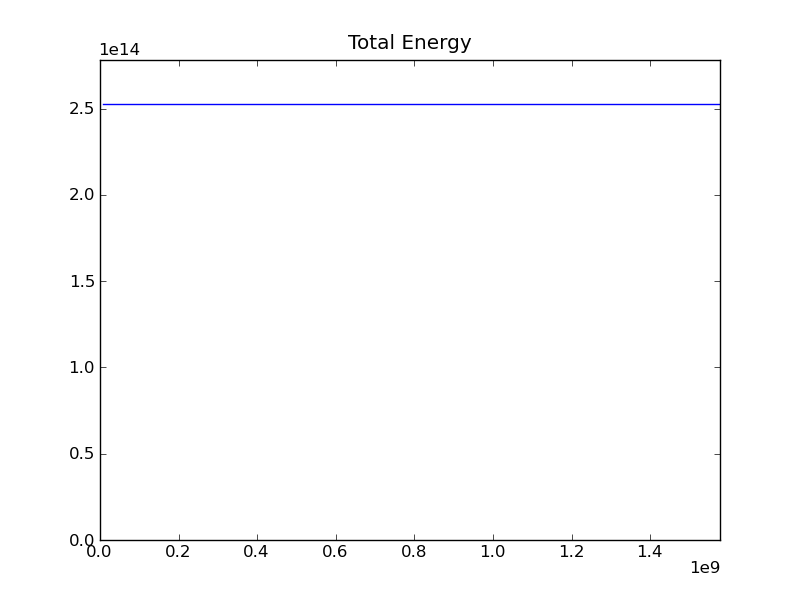
\includegraphics[width=4in]{figures/ttblockspyplot150}
\caption{Total Energy in the Blocks over Time (in seconds).}
\label{fig:onedheatout1} 
\end{center}
\end{figure}

\subsection{Plotting the Total Energy} 
\sslist{onedheatdiff001.py}

\esc does not include its own plotting capabilities. However, it is possible to use a variety of free \pyt packages for visualisation.
Two types will be demonstrated in this cookbook; \mpl\footnote{\url{http://matplotlib.sourceforge.net/}} and \verb VTK \footnote{\url{http://www.vtk.org/}} visualisation. 
The \mpl package is a component of SciPy\footnote{\url{http://www.scipy.org}} and is good for basic graphs and plots. 
For more complex visualisation tasks in particular when it comes to  two and three dimensional problems it is recommended to us more advanced tools for instance  \mayavi \footnote{\url{http://code.enthought.com/projects/mayavi/}}
which bases on the \verb|VTK| toolkit. We will discuss the usage of \verb|VTK| based 
visualization in Chapter~\ref{Sec:2DHD} where will discuss a two dimensional PDE. 

For our simple problem we have two plotting tasks: Firstly we are interested in showing the
behaviour of the total energy over time and secondly in how the temperature distribution within the block is 
developing over time. Lets start with the first task.

The trick is to create a record of the time marks and the corresponding total energies observed.
\pyt provides the concept of lists for this. Before 
the time loop is opened we create empty lists for the time marks \verb|t_list| and the total energies \verb|E_list|. 
After the new temperature as been calculated by solving the PDE we append the new time marker and total energy
to the corresponding list using the \verb|append| method. With these modifications the script looks as follows:
\begin{python}
t_list=[]
E_list=[]
# ... start iteration:
while t<tend:
      t+=h
      mypde.setValue(Y=qH+rhocp/h*T) # set variable PDE coefficients
      T=mypde.getSolution() #get the PDE solution
      totE=integrate(rhocp*T) 
      t_list.append(t)   # add current time mark to record
      E_list.append(totE) # add current total energy to record
\end{python}
To plot $t$ over $totE$ we use the \mpl a module contained within \pylab which needs to be loaded before used;
\begin{python}
import pylab as pl # plotting package.
\end{python}
Here we are not using the \verb|from pylab import *| in order to avoid name clashes for function names 
within \esc. 

The following statements are added to the script after the time loop has been completed;
\begin{python}
pl.plot(t_list,E_list)
pl.title("Total Energy")
pl.axis([0,max(t_list),0,max(E_list)*1.1])
pl.savefig("totE.png")
\end{python}
The first statement hands over the time marks and corresponding total energies to the plotter. 
The second statment is setting the title for the plot. The third statement
sets the axis ranges. In most cases these are set appropriately by the plotter.  
The last statement renders the plot and writes the 
result into the file \verb|totE.png| which can be displayed by (almost) any image viewer. 
As expected the total energy is constant over time, see \reffig{fig:onedheatout1}.

\subsection{Plotting the Temperature Distribution}
\sslist{onedheatdiff001b.py}
For plotting the spatial distribution of the temperature we need to modify the strategy we have used
for the total energy. Instead of producing a final plot at the end we will generate a 
picture at each time step which can be browsed as slide show or composed to a movie.
The first problem we encounter is that if we produce an image in each time step we need
to make sure that the images previously generated are not overwritten.

To develop an incrementing file name we can use the following convention. It is convenient to
put all image file showing the same variable - in our case the temperature distribution -
into a separate directory. As part of the \verb|os| module\footnote{The \texttt{os} module provides 
a powerful interface to interact with the operating system, see \url{http://docs.python.org/library/os.html}.} \pyt 
provides the  \verb|os.path.join| command to build file and
directory names in a platform independent way. Assuming that 
\verb|save_path| is name of directory we want to put the results the command is; 
\begin{python}
import os
os.path.join(save_path, "tempT%03d.png"%i )
\end{python}
where \verb|i| is the time step counter.
There are two arguments to the \verb join  command. The \verb save_path  variable is a predefined string pointing to the directory we want to save our data in, for example a single sub-folder called \verb data  would be defined by;
\begin{verbatim}
save_path = "data"
\end{verbatim}
while a sub-folder of \verb data  called \verb onedheatdiff001  would be defined by;
\begin{verbatim}
save_path = os.path.join("data","onedheatdiff001")
\end{verbatim}
The second argument of \verb join \xspace contains a string which is the file name or subdirectory name. We can use the operator \verb|%| to increment our file names with the value \verb|i| denoting a incrementing counter. The sub-string \verb %03d  does this by defining the following parameters; 
\begin{itemize}
 \item \verb 0  becomes the padding number;
 \item \verb 3  tells us the amount of padding numbers that are required; and
 \item \verb d  indicates the end of the \verb %  operator.
\end{itemize}
To increment the file name a \verb %i  is required directly after the operation the string is involved in. When correctly implemented the output files from this command would be place in the directory defined by \verb save_path  as;
\begin{verbatim}
blockspyplot.png
blockspyplot.png
blockspyplot.png
...
\end{verbatim}
and so on.

A sub-folder check/constructor is available in \esc. The command;
\begin{verbatim}
mkDir(save_path)
\end{verbatim}
will check for the existence of \verb save_path  and if missing, make the required directories.

We start by modifying our solution script from before.
Prior to the \verb|while| loop we will need to extract our finite solution points to a data object that is compatible with \mpl. First we create the node coordinates of the sample points used to represent
the temperature as a \pyt list of tuples or a \numpy array as requested by the plotting function. 
We need to convert thearray \verb|x| previously set as \verb|Solution(blocks).getX()| into a \pyt list 
and then to a \numpy array. The $x\hackscore{0}$ component is then extracted via an array slice to the variable \verb|plx|; 
\begin{python}
import numpy as np # array package.
#convert solution points for plotting
plx = x.toListOfTuples() 
plx = np.array(plx) # convert to tuple to numpy array
plx = plx[:,0] # extract x locations
\end{python}

\begin{figure}
\begin{center}
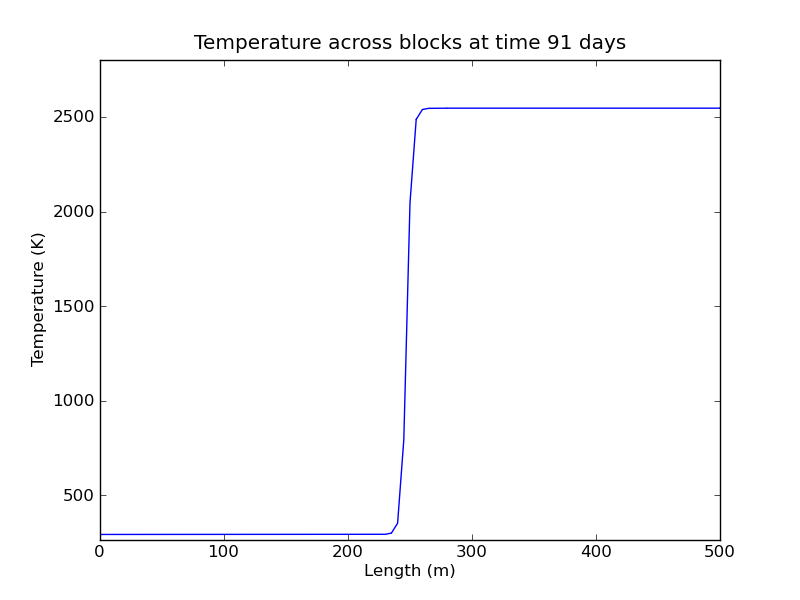
\includegraphics[width=4in]{figures/blockspyplot001}
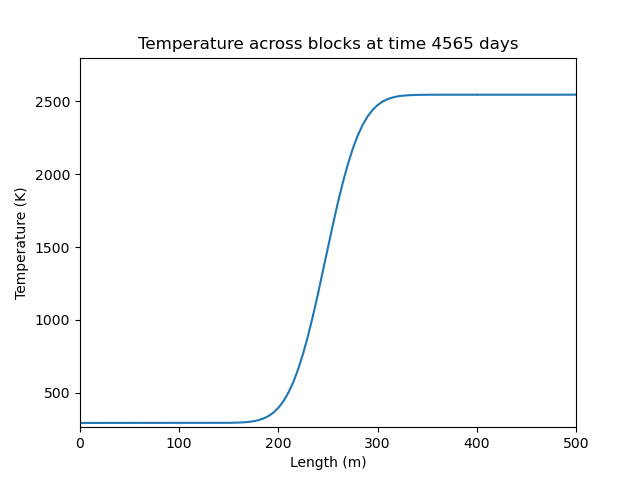
\includegraphics[width=4in]{figures/blockspyplot050}
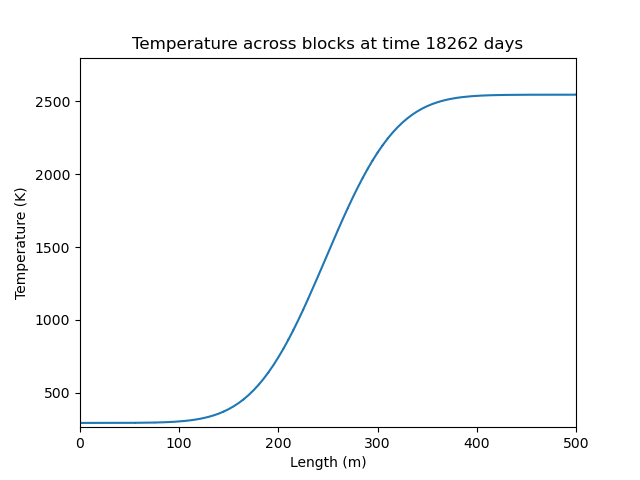
\includegraphics[width=4in]{figures/blockspyplot200}
\caption{Temperature ($T$) distribution in the blocks at time steps $1$, $50$ and $200$.}
\label{fig:onedheatout} 
\end{center}
\end{figure}

For each time step we will generate a plot of the temperature distribution and save each to a file. We use the same
techniques provided by \mpl as we have used to plot the total energy over time.
The following is appended to the end of the \verb while  loop and creates one figure of the temperature distribution. We start by converting the solution to a tuple and then plotting this against our \textit{x coordinates} \verb plx  we have generated before. We add a title to the diagram before it is rendered into a file. 
Finally, the figure is saved to a \verb|*.png| file and cleared for the following iteration.
\begin{python}
# ... start iteration:
while t<tend:
        ....
	T=mypde.getSolution() #get the PDE solution
        tempT = T.toListOfTuples() # convert to a tuple
        pl.plot(plx,tempT) # plot solution
	# set scale (Temperature should be between Tref and T0)
        pl.axis([0,mx,Tref*.9,T0*1.1])
        # add title
	pl.title("Temperature across the blocks at time %e minutes"%(t/day))
	#save figure to file
	pl.savefig(os.path.join(save_path,"tempT","blockspyplot%03d.png") %i)
\end{python}
Some results are shown in \reffig{fig:onedheatout}. 

\subsection{Make a video} 
Our saved plots from the previous section can be cast into a video using the following command appended to the end of the script. \verb mencoder  is Linux only however, and other platform users will need to use an alternative video encoder.
\begin{python}
# compile the *.png files to create a *.avi videos that show T change
# with time. This operation uses Linux mencoder. For other operating 
# systems it is possible to use your favourite video compiler to
# convert image files to videos.

os.system("mencoder mf://"+save_path+"/tempT"+"/*.png -mf type=png:\
           w=800:h=600:fps=25 -ovc lavc -lavcopts vcodec=mpeg4 -oac copy -o \
           onedheatdiff001tempT.avi")
\end{python}
 


%%%%%%%%%%%%%%%%%%%%%%%%%%%%%%%%%%%%%%%%%%%%%%%%%%%%%%%%
%
% Copyright (c) 2003-2009 by University of Queensland
% Earth Systems Science Computational Center (ESSCC)
% http://www.uq.edu.au/esscc
%
% Primary Business: Queensland, Australia
% Licensed under the Open Software License version 3.0
% http://www.opensource.org/licenses/osl-3.0.php
%
%%%%%%%%%%%%%%%%%%%%%%%%%%%%%%%%%%%%%%%%%%%%%%%%%%%%%%%%

\section{One Dimensional Heat Diffusion accross an Interface}
\sslist{onedheatdiff002.py and cblib.py}
%\label{Sec:1DHDv1}
 It is quite simple to now expand upon the 1D heat diffusion problem we just tackled. Suppose we have two blocks of isotropic material which are very large in all directions to the point that the interface between the two blocks appears infinite in length compared to the distance we are modelling perpendicular to the interface and accross the two blocks. If \textit{Block 1} is of a temperature \verb 0  and \textit{Block 2} is at a temperature \verb T  what would happen to the temperature distribution in each block if we placed them next to each other. This problem is very similar to our Iron Rod but instead of a constant heat source we instead have a heat disparity with a fixed amount of energy. In such a situation it is common knowledge that the heat energy in the warmer block will gradually conduct into the cooler block until the temperature between the blocks is balanced.

\begin{figure}[h!]
\centerline{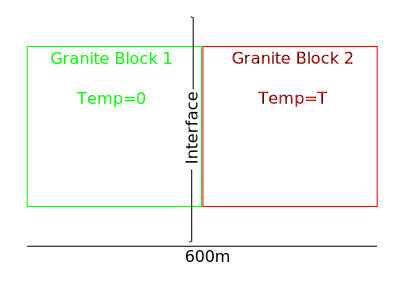
\includegraphics[width=4.in]{figures/onedheatdiff002}}
\caption{Temperature differential along a single interface between two granite blocks.}
\label{fig:onedgbmodel}
\end{figure}

By modifying our previous code it is possible to solve this new problem. In doing so we will also try to tackle a real world example and as a result, introduce and discuss some new variables. The linear model of the two blocks is very similar to the effect a large magmatic intrusion would have on a cold country rock. It is however, simpler at this stage to have both materials the same and for this example we will use granite \reffig{fig:onedgbmodel}.  The intrusion will have an initial temperature defined by \verb Tref  and the granite properties required are:
\begin{python}
#PDE related
mx = 500*m #meters - model length
my = 100*m #meters - model width
ndx = 500 # mesh steps in x direction 
ndy = 1 # mesh steps in y direction
boundloc = mx/2 # location of boundary between two blocks
q=0.*Celsius #our heat source temperature is now zero
Tref=2273.*Celsius # Kelvin -the starting temperature of our RHS Block
rho = 2750*kg/m**3 #kg/m^{3} density of granite
cp = 790.*J/(kg*K) #j/Kg.K thermal capacity
rhocp = rho*cp	#DENSITY * SPECIFIC HEAT
eta=0.  # RADIATION CONDITION
kappa=2.2*W/m/K #watts/m.K thermal conductivity
\end{python}

Since the scale and values involved in our problem have changed, the length and step size of the iteration must be considered. Instead of seconds which our units are in, it may be more prudent to decide the number of days or years we would like to run the simulation over.
\begin{python}
#Script/Iteration Related
t=0. #our start time, usually zero
tend=10*yr #the time we want to end the simulation in years
outputs = 400 # number of time steps required.
h=(tend-t)/outputs #size of time step
\end{python}

If we assume that the dimensions of the blocks are continuous and extremely large compared with the model size then we need only model a small proportion of the boundary. It is practical to locate the boundary between the two blocks at the center of our model. As there is no heat source our \verb q  variable can be set to zero. The new initial conditions are defined using the following:
\begin{python}
#establish location of boundary between two blocks
bound = x[0]-boundloc
#set initial temperature
T= 0*Tref*whereNegative(bound)+Tref*wherePositive(bound)
\end{python}
The \verb bound statement sets the boundary to the location along the \textit{x-axis} defined by \verb boundloc  .
The PDE can then be solved as before.

FOR THE READER:
\begin{enumerate}
 \item Move the boundary line between the two blocks to another part of the domain.
 \item Try splitting the domain in to multiple blocks with varying temperatures.
\end{enumerate}



%%%%%%%%%%%%%%%%%%%%%%%%%%%%%%%%%%%%%%%%%%%%%%%%%%%%%%%%
%
% Copyright (c) 2003-2010 by University of Queensland
% Earth Systems Science Computational Center (ESSCC)
% http://www.uq.edu.au/esscc
%
% Primary Business: Queensland, Australia
% Licensed under the Open Software License version 3.0
% http://www.opensource.org/licenses/osl-3.0.php
%
%%%%%%%%%%%%%%%%%%%%%%%%%%%%%%%%%%%%%%%%%%%%%%%%%%%%%%%%

\begin{figure}[t]
\centerline{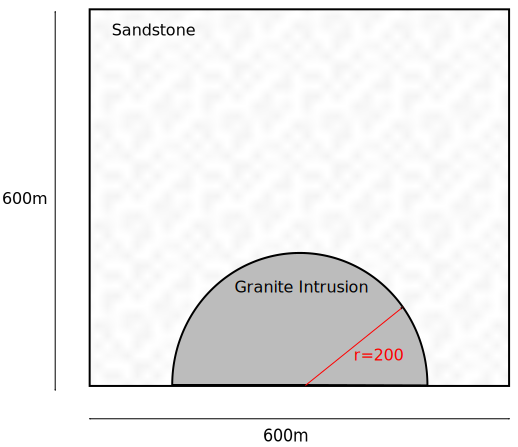
\includegraphics[width=4.in]{figures/twodheatdiff}}
\caption{2D model: granitic intrusion of sandstone country rock.}
\label{fig:twodhdmodel}
\end{figure}

\sslist{twodheatdiff001.py and cblib.py}

Building upon our success from the 1D models, it is now prudent to expand our domain by another dimension. 
For this example we will be using a very simple magmatic intrusion as the basis for our model. The simulation will be a single event where some molten granite has formed a cylindrical dome at the base of some cold sandstone country rock. Assuming that the cylinder is very long 
we model a cross-section as shown in \reffig{fig:twodhdmodel}. We will implement the same 
diffusion model as we have use for the granite blocks in \refSec{Sec:1DHDv00}
but will add the second spatial dimension and show how to define 
variables depending on the location of the domain. 
We use \file{onedheatdiff001b.py} as the starting point for develop this model. 

\section{Two Dimensional Heat Diffusion for a basic Magmatic Intrusion}
\label{Sec:2DHD}

To expand upon our 1D problem, the domain must first be expanded. In fact, we have solved a two dimensional problem already but didn't put much 
attention to the second dimension. This will be changed now. 
In our definition phase by creating a square domain in $x$ and $y$\footnote{In \esc the notation
$x\hackscore{0}$ and $x\hackscore{1}$ is used for $x$ and $y$, respectively.} that is $600$ meters along each side \reffig{fig:twodhdmodel}. The number of discrete spatial cells will be 100 in either direction. The radius of the intrusion will be $200$ meters with the centre located at the $300$ meter mark on the $x$-axis. The domain variables are;
\begin{python}
mx = 600*m #meters - model length
my = 600*m #meters - model width
ndx = 150 #mesh steps in x direction 
ndy = 150 #mesh steps in y direction
r = 200*m #meters - radius of intrusion
ic = [300*m, 0] #coordinates of the centre of intrusion (meters)
qH=0.*J/(sec*m**3) #our heat source temperature is zero
\end{python}
As before we use 
\begin{python}
model = Rectangle(l0=mx,l1=my,n0=ndx, n1=ndy)
\end{python}
to generate the domain. 

There are two fundamental changes to the PDE has we have discussed PDEs in \refSec{Sec:1DHDv00}. Firstly,
as the material coefficients for granite and sandstone is different, we need to deal with 
PDE coefficients which vary with there location in the domain. Secondly, we need 
to deal with the second spatial dimension. We will look at these two modification at the same time. 
In fact our temperature model \refEq{eqn:hd} we have used in \refSec{Sec:1DHDv00} applies for the 
1D case with constant material parameter only. For the more general case we are interested 
in this chapter the correct model equation is 
\begin{equation}
\rho c\hackscore p \frac{\partial T}{\partial t} -  \frac{\partial }{\partial x} \kappa \frac{\partial T}{\partial x} -  \frac{\partial }{\partial y} \kappa \frac{\partial T}{\partial y} = q\hackscore H 
\label{eqn:hd2}
\end{equation}
Notice, that for the 1D case we have $\frac{\partial T}{\partial y}=0$ and
for the case of constant material parameters $\frac{\partial }{\partial x} \kappa = \kappa  \frac{\partial }{\partial x}$ so this new equation coincides with simplified model equation for this case. It is more convenient 
to write this equation using the $\nabla$ notation as we have already seen in \refEq{eqn:commonform nabla};
\begin{equation}\label{eqn:Tform nabla}
\rho c\hackscore p \frac{\partial T}{\partial t} 
-\nabla \cdot \kappa \nabla T = q\hackscore H
\end{equation}
We can easily apply the backward Euler scheme as before to end up with 
\begin{equation}
\frac{\rho c\hackscore p}{h} T^{(n)} -\nabla \cdot \kappa \nabla T^{(n)}  = q\hackscore H +  \frac{\rho c\hackscore p}{h} T^{(n-1)}
\label{eqn:hdgenf2}
\end{equation}
which is very similar to \refEq{eqn:hdgenf} used to define the temperature update in the simple 1D case. 
The difference is in the second order derivate term $\nabla \cdot \kappa \nabla T^{(n)}$. Under 
the light of the more general case we need to revisit the \esc PDE form as 
shown in \ref{eqn:commonform2D}. For the 2D case with variable PDE coefficients 
the form needs to be read as 
\begin{equation}\label{eqn:commonform2D 2}
-\frac{\partial }{\partial x} A\hackscore{00}\frac{\partial u}{\partial x} 
-\frac{\partial }{\partial x} A\hackscore{01}\frac{\partial u}{\partial y} 
-\frac{\partial }{\partial y} A\hackscore{10}\frac{\partial u}{\partial x} 
-\frac{\partial }{\partial x} A\hackscore{11}\frac{\partial u}{\partial y} 
+ Du = f
\end{equation}
So besides the settings $u=T^{(n)}$, $D = \frac{\rho c \hackscore{p}}{h}$ and
$f = q \hackscore{H} + \frac{\rho c\hackscore p}{h} T^{(n-1)}$ as we have used before (see \refEq{ESCRIPT SET}) we need to set
\begin{equation}\label{eqn: kappa general}
A\hackscore{00}=A\hackscore{11}=\kappa; A\hackscore{01}=A\hackscore{10}=0
\end{equation}
The fundamental difference to the 1D case is that $A\hackscore{11}$ is not set to zero but $\kappa$ 
which brings in the second dimension. Important to notice that the fact that the coefficients 
of the PDE may depend on their location in the domain now does not influence the usage of the PDE form. This is very convenient as we can introduce spatial dependence to the PDE coefficients without modification to the way we call the PDE solver. 

A very convenient way to define the matrix $A$ is required in \refEq{eqn: kappa general} is using the 
Kronecker $\delta$ symbol\footnote{see \url{http://en.wikipedia.org/wiki/Kronecker_delta}}. The 
\esc function \verb|kronecker| returns this matrix;
\begin{equation}
\verb|kronecker(model)| = \left[ 
\begin{array}{cc}
 1 & 0 \\
 0 & 1 \\
\end{array}
\right]
\end{equation}
As the argument \verb|model| represents a two dimensional domain the matrix is returned as $2 \times 2$ matrix
(In case of a three-dimensional domain a $3 \times 3$ matrix is returned). The call 
\begin{python}
mypde.setValue(A=kappa*kronecker(model),D=rhocp/h)
\end{python}
sets the PDE coefficients according to \refEq{eqn: kappa general}.  

Before we turn the question how we set $\kappa$ we need to check the boundary conditions. As
pointed out in \refEq{NEUMAN 2} makes certain assumptions on the boundary conditions. In our case
this assumptions translates to;
\begin{equation}
-n\hackscore{0} \cdot \kappa \frac{\partial T^{(n)}}{\partial x} - n\hackscore{1} \cdot  \kappa \frac{\partial T^{(n)}}{\partial y} = 0
\end{equation}
which sets the normal component of the heat flux $- \kappa \cdot (\frac{\partial T^{(n)}}{\partial x}, \frac{\partial T^{(n)}}{\partial y})$ to zero. This means that the regions is insulated which is what we want. 
On the left and right face of the domain where we have $(n\hackscore{0},n\hackscore{1} ) = (\mp 1,0)$ 
this means $\frac{\partial T^{(n)}}{\partial x}=0$ and on the top and bottom on the domain 
where we have  $(n\hackscore{0},n\hackscore{1} ) = (\pm 1,0)$ this is $\frac{\partial T^{(n)}}{\partial y}=0$. 

\section{Setting Variable PDE Coefficients}
Now we need to look into the problem how we define the material coefficients
$\kappa$ and $\rho c\hackscore p$ depending on there location in the domain. 
We have used the technique we discuss here already when we set up the initial
temperature in the granite block example in \refSec{Sec:1DHDv00}. However,
the situation is more complicated here as we have to deal with a
curved interface between the two sub-domain.

Prior to setting up the PDE the interface between the two materials must be established. 
The distance $s\ge 0$ between two points $[x,y]$ and $[x\hackscore{0},y\hackscore{0}]$ in Cartesian coordinates is defined as:
\begin{equation}
 (x-x\hackscore{0})^{2}+(y-y\hackscore{0})^{2} = s^{2}
\end{equation}
If we define the point $[x\hackscore{0},y\hackscore{0}]$ as $ic$ which denotes the centre of the semi-circle of our intrusion, then for all the points $[x,y]$ in our model we can calculate a distance to $ic$. 
All the points that fall within the given radius $r$ of our intrusion will have a corresponding 
value $s < r$ and all those belonging to the country rock will have a value $s > r$. By subtracting $r$ from both of these conditions we find $s-r < 0$ for all intrusion points and $s-r > 0$ 
for all country rock points. 
Defining these conditions within the script is quite simple and is done using the following command:
\begin{python}
 bound = length(x-ic)-r #where the boundary will be located
\end{python}
This definition of the boundary can now be used with \verb|whereNegative| command again to help define the material constants and temperatures in our domain. 
If \verb|kappai| and \verb|kappac| are the 
thermal conductivities for the intrusion material granite and for the surrounding sandstone we set; 
\begin{python}
x=Function(model).getX()
bound = length(x-ic)-r
kappa = kappai * whereNegative(bound) + kappac * (1-whereNegative(bound))
mypde.setValue(A=kappa*kronecker(model))
\end{python}
Notice that we are using the sample points of the \verb|Function| function space as expected for the 
PDE coefficient \verb|A|\footnote{For the experience user: use \texttt{x=mypde.getFunctionSpace("A").getX()}.}
The corresponding statements are used to set $\rho c\hackscore p$. 

Our PDE has now been properly established. The initial conditions for temperature are set out in a similar matter:
\begin{python}
#defining the initial temperatures.
x=Solution(model).getX()
bound = length(x-ic)-r
T= Ti*whereNegative(bound)+Tc*(1-whereNegative(bound))
\end{python}
where \verb|Ti| and \verb|Tc| are the initial temperature
in the regions of the granite and surrounding sandstone, respectively. It is important to
notice that we have reset \verb|x| and \verb|bound| to refer to the appropriate 
sample points of a PDE solution\footnote{For the experience user: use \texttt{x=mypde.getFunctionSpace("r").getX()}.}.

\begin{figure}[h]
\centerline{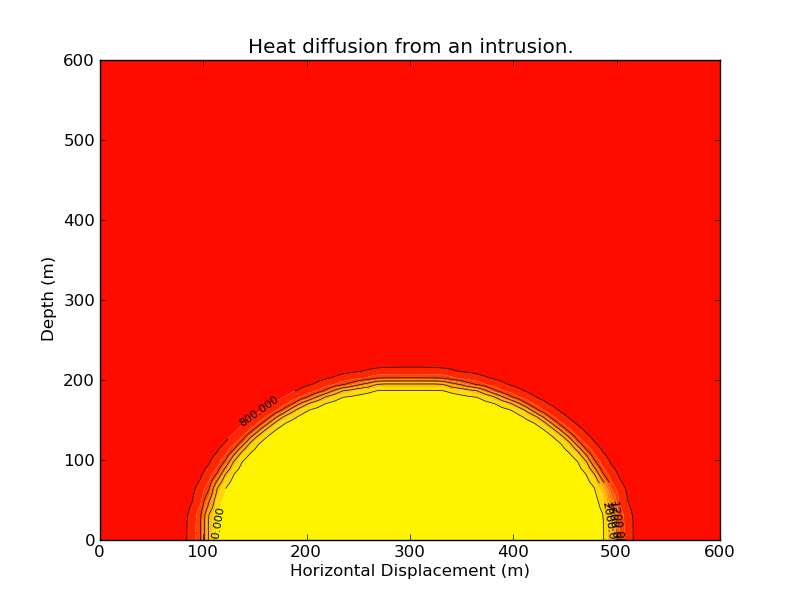
\includegraphics[width=4.in]{figures/heatrefraction001.png}}
\centerline{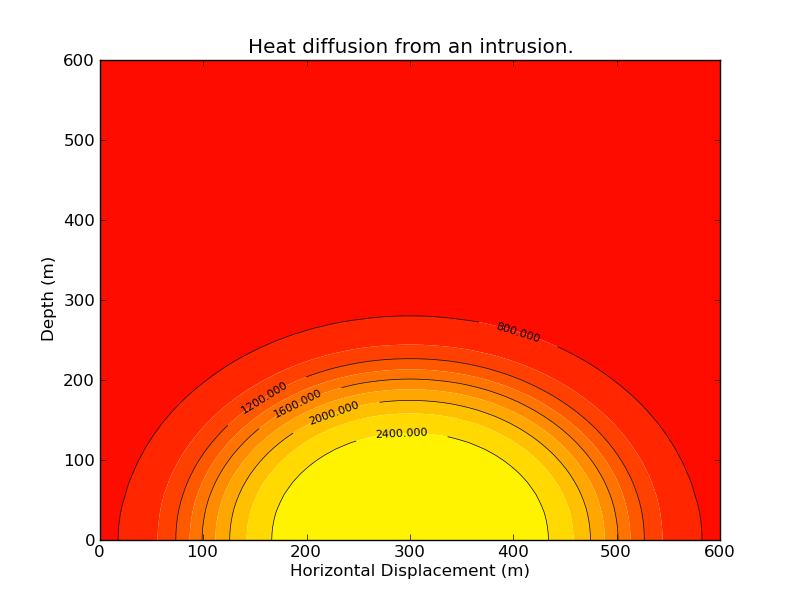
\includegraphics[width=4.in]{figures/heatrefraction030.png}}
\centerline{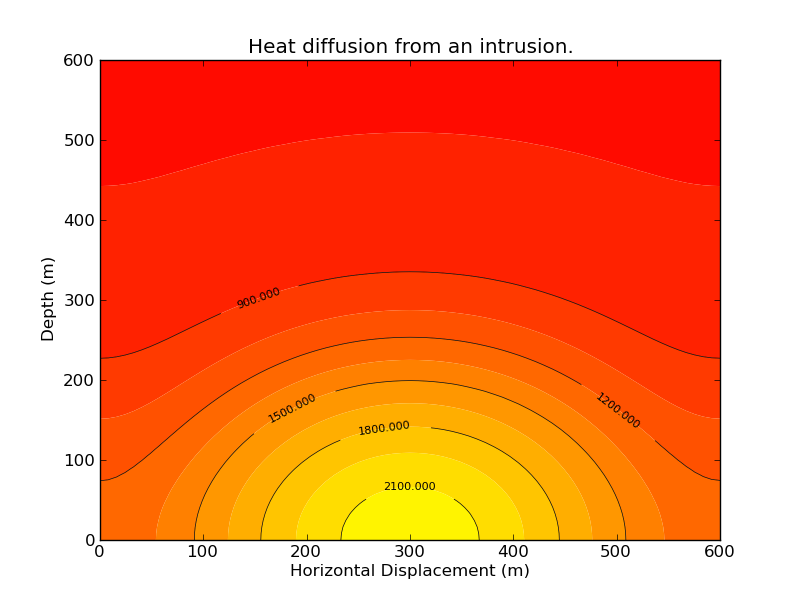
\includegraphics[width=4.in]{figures/heatrefraction200.png}}
\caption{2D model: Total temperature distribution ($T$) at time step $1$, $20$ and $200$. Contour lines show temperature.}
\label{fig:twodhdans}
\end{figure}

\section{Contouring \esc data using \modmpl.}
To complete our transition from a 1D to a 2D model we also need to modify the 
plotting procedure. As before we use the  \modmpl to do the plotting 
in this case a contour plot. For 2D contour plots \modmpl expects that the
data are regularly gridded. We have no control on the location and ordering of the sample points
used to represent the solution. Therefore it is necessary to interpolate our solution onto a regular grid.

In \refSec{sec: plot T} we have already learned how to extract the $x$ coordinates of sample points as 
\verb|numpy| array to hand the values to \modmpl. This can easily be extended to extract both the
$x$ and the $y$ coordinates;
\begin{python}
import numpy as np
def toXYTuple(coords):
    coords = np.array(coords.toListOfTuples()) #convert to Tuple
    coordX = coords[:,0] #X components.
    coordY = coords[:,1] #Y components.
    return coordX,coordY
\end{python}
For convenience we have put this function into \file{clib.py} file so we can use this
function in other scripts more easily. 


We now generate a regular $100 \times 100$ grid over the domain ($mx$ and $my$ 
are the dimensions in $x$ and $y$ direction) which is done using the \modnumpy function \verb|linspace|  . 
\begin{python}
from clib import toXYTuple
# get sample points for temperature as  for contouring      
coordX, coordY = toXYTuple(T.getFunctionSpace().getX())
# create regular grid
xi = np.linspace(0.0,mx,75)
yi = np.linspace(0.0,my,75)
\end{python}
The values \verb|[xi[k], yi[l]]| are the grid points.

The remainder of our contouring commands reside within a \verb while  loop so that a new contour is generated for each time step. For each time step the solution must be regridded for \modmpl using the \verb griddata  function. This function interprets a potentially irregularly located values \verb tempT  at locations defined by \verb coordX  and \verb coordY as values at the new coordinates of a rectangular grid defined by
\verb xi   and \verb yi . The output is \verb zi  . It is now possible to use the \verb contourf  function which generates colour filled contours. The colour gradient of our plots is set via the command \verb pl.matplotlib.pyplot.autumn() , other colours are listed on the \modmpl web page\footnote{see \url{http://matplotlib.sourceforge.net/api/}}. Our results are then contoured, visually adjusted using the \modmpl functions and then saved to file. \verb pl.clf()  clears the figure in readiness for the next time iteration.
\begin{python}
#grid the data.
zi = pl.matplotlib.mlab.griddata(coordX,coordY,tempT,xi,yi)
# contour the gridded data, plotting dots at the randomly spaced data points.
pl.matplotlib.pyplot.autumn()
pl.contourf(xi,yi,zi,10)
CS = pl.contour(xi,yi,zi,5,linewidths=0.5,colors='k')
pl.clabel(CS, inline=1, fontsize=8)
pl.axis([0,600,0,600])
pl.title("Heat diffusion from an intrusion.")
pl.xlabel("Horizontal Displacement (m)")
pl.ylabel("Depth (m)")
pl.savefig(os.path.join(save_path,"heatrefraction%03d.png") %i)
pl.clf()        
\end{python}
The function \verb|pl.contour| is used to add labeled contour lines to the plot. 
The results for selected time steps are shown in \reffig{fig:twodhdans}.



\section{Advanced Visualization using VTK}

\sslist{twodheatdiffvtk.py}
An alternative approach to \modmpl for visualization is the usage of a package which base on 
visualization tool kit (VTK) library\footnote{see \url{http://www.vtk.org/}}. There is a variety 
of package available. Here we will use the package \mayavi\footnote{see \url{http://code.enthought.com/projects/mayavi/}} as an example. 

\mayavi is an interactive, GUI driven tool which is 
really designed to visualize large three dimensional data sets where \modmpl 
is not suitable. But it is very useful when it comes to two dimensional problems. 
The decision which tool is best is finally the user's decision. The main 
difference between using \mayavi (and other VTK based tools)
or \modmpl is the fact that actually visualization is detached from the 
calculation by writing the results to external files
and import them into \mayavi. In 3D where the best camera position for rendering a scene is not obvious 
before the results are available. Therefore the user may need to try 
different position before the best is found. Moreover, in many cases in 3D the interactive 
visualization is the only way to really understand the results (e.g. using stereographic projection). 

To write the temperatures at each time step to data files in the VTK file format one
needs to insert a \verb|saveVTK| call into the code;
\begin{python}
while t<=tend:
      i+=1 #counter
      t+=h #current time
      mypde.setValue(Y=qH+T*rhocp/h)
      T=mypde.getSolution()
      saveVTK(os.path.join(save_path,"data.%03d.vtu"%i, T=T)
\end{python}
The data files, eg. \file{data.001.vtu}, contains all necessary information to 
visualize the temperature and can directly processed by \mayavi. Notice that there is no 
regridding required. It is recommended to use the file extension \file{.vtu} for files
created by \verb|saveVTK|. 

\begin{figure}[h]
\centerline{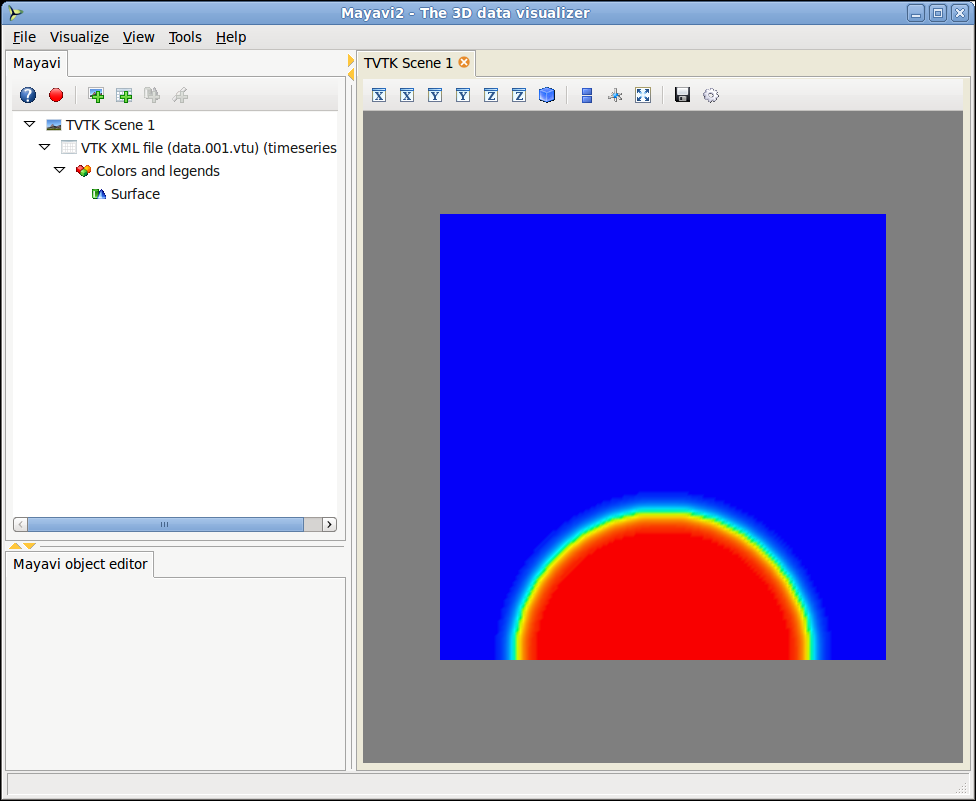
\includegraphics[width=4.in]{figures/ScreeshotMayavi2n1}}
\caption{\mayavi start up Window.}
\label{fig:mayavi window}
\end{figure}

\begin{figure}[h]
\centerline{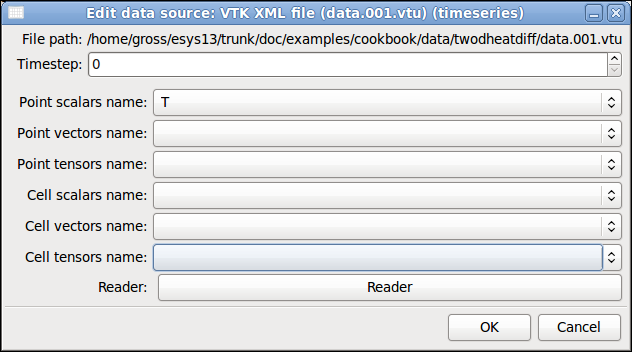
\includegraphics[width=4.in]{figures/ScreeshotMayavi2n2}}
\caption{\mayavi data control window.}
\label{fig:mayavi window2}
\end{figure}
After you have run the script you will find the 
result files \file{data.*.vtu} in the result directory \file{data/twodheatdiff}. Run the 
command
\begin{python}
>> mayavi2 -d data.001.vtu -m Surface &
\end{python}
from the result directory. \mayavi will start up a window similar to \reffig{fig:mayavi window}.
The right hand side shows the temperature at the first time step. To show
the results at other time steps you can click at the item \texttt{VTK XML file (data.001.vtu) (timeseries)}
at the top left hand side. This will bring up a new window similar to tye window shown in  \reffig{fig:mayavi window2}. By clicking at the arrows in the top right corner you can move forwards and backwards in time. 
You will also notice the text \textbf{T} next to the item \texttt{Point scalars name}. The
name \textbf{T} corresponds to the keyword argument name \texttt{T} we have used 
in the \verb|saveVTK| call. In this menu item you can select other results 
you may have written to the output file for visualization.

\textbf{For the advanced user}: Using the \modmpl to visualize spatially distributed data 
is not MPI compatible. However, the \verb|saveVTK| function can be used with MPI. In fact,
the function collects the values of the sample points spread across processor ranks into a single.
For more details on writing scripts for parallel computing please consult the \emph{user's guide}.

% Moving into 2D and 3D wave propagations in next chapters.
\chapter{Seismic Wave Propagation}

%%%%%%%%%%%%%%%%%%%%%%%%%%%%%%%%%%%%%%%%%%%%%%%%%%%%%%%%
%
% Copyright (c) 2003-2009 by University of Queensland
% Earth Systems Science Computational Center (ESSCC)
% http://www.uq.edu.au/esscc
%
% Primary Business: Queensland, Australia
% Licensed under the Open Software License version 3.0
% http://www.opensource.org/licenses/osl-3.0.php
%
%%%%%%%%%%%%%%%%%%%%%%%%%%%%%%%%%%%%%%%%%%%%%%%%%%%%%%%%

\section{Seismic Wave Propagation in Two Dimensions}
\editor{This chapter aims to expand the readers understanding of escript by modelling the wave equations.
Challenges will include a second order differential (multiple initial conditions). A new PDE to fit to the general form. Movement to a 3D problem (maybe)??? }

\verb|wavesolver2d.py|

Wave propagation in the earth can be described by the wave equation:
\begin{equation} \label{eqn:wav} \index{wave equation}
\rho \frac{\partial^{2}u\hackscore{i}}{\partial t^2} - \frac{\partial \sigma\hackscore{ij}}{\partial\hackscore{j}} = 0
\end{equation}
where $\sigma$ represents stress and is given by:
\begin{equation} \label{eqn:sigw}
 \sigma \hackscore{ij} = \lambda u\hackscore{k,k} \delta\hackscore{ij} + \mu ( u\hackscore{i,j} + u\hackscore{j,i})
\end{equation}
$\lambda$ and $\mu$ are the Lame Coefficients. Specifically $\mu$ is the bulk modulus. Equation \ref{eqn:wav} can be written with the Einstein summation convention as:
\begin{equation}
 \rho u\hackscore{i,tt} = \sigma\hackscore{ij,j}
\end{equation}
For this model we will specify the boundary conditions such that the normal of the stress from the boundary is zero.
\begin{eqnarray} \label{eqn:bdw}
\sigma \hackscore{ij}n\hackscore{j}=0
\end{eqnarray}
To solve this PDE we are going to write a more generic solution routine than we have in the previous chapters. There are a number of advantages to this approach. Firstly, by writing a subroutine that will solve a 2D wave propagation problem it reduces the amount of code duplication that may occur. When errors arrise one need only ammend the subroutine rather than all iterations of it that may have been created. This saves time and effort in the long run. 

To create the our subroutine we will need to import all our necessary libraries again. This is as for previous examples. Then we can define our script and the variables it will take. Our subroutine is located in \verb|/examples/cblib/wavesolver2d.py|  . The arguments of the subroutine are;
\begin{verbatim}
domain  : domain to solve over
h       : time step
tend    : end time
lam, mu : lames constants for domain
rho	: density of domain
U0	: magnitude of source
xc	: source location in domain (Vector)
savepath: where to output the data files
\end{verbatim}
There are a few differences between the wave equation and the heat diffusion problem of the previous chapter. While the nodes are defined the same way with the function \verb getX  and the PDE is still linear; one must consider the solution method. Without the line;
\begin{verbatim}
mypde.setSolverMethod(LinearPDE.LUMPING)
\end{verbatim}
the PDE would take a significant amount of time to solve. The \verb LUMPING  functionality implements an aggressive approximation for the $D$ coefficient matrix of the \esc linear PDE general form. While \verb LUMPING  introduces additional error to the solution it can significantly reduce the solution time. Care should be taken however, as this function can only be used when the $A$, $B$ and $C$ coefficients of the general form are zero. 

As the wave equation has a double time derivative, it is not sufficient to only stipulate the initial conditions for one time step. Two time steps must be specified so that the equation can be solved. For this example $u$ (\verb u ) and $u(t-1)$ (\verb u_m1 ) will be the same but if both of these condititions are known, they can be specified individually. It should be noted here that if multiple time steps are known at the begining of a model, they can be added to the simulation manually. The solver can then continue the model from the end of the known data. Alternatively, if the source motion is understood, its position can be corrected for each iteration to create a more accurate recreation of an event. 

The source in this example will induce a radially propagating wave. A small displacement will be applied to the medium about a singularity which we have called \verb xc  , this is the source location. We start by giving the source some spatial magnitude by defining a small radius about \verb xc  which is affected. The \verb src_radius  needs to cover a significant portion of grid nodes, otherwise the waves generated will suffer from dispersion due to an inadequate grid step size. If the source is small, the grid stepping must reflect the size of the source for more accurate results. Our radius will be;
\begin{verbatim}
 src_radius = 50
\end{verbatim}
Now that the extent of the source has been allocated it needs two more things; a direction and a magnitude. We can choose a direction based on the 360 degrees that exist in a full circle. If we take $\theta=0$ to be the x-axis and move counter clockwise then we can create a directional vector $U=[dx,dy]$  where $tan(\theta) = dy/dx$. It is also necessary to ensure that our directional vector of unit length such that $|U|=1$; which implies $\sqrt{dx^2+dy^2}=1$. By doing this we ensure that no accidental scaling is introduced to our source term. Here are three examples of different directions which satisfy the above conditions;
\begin{enumerate}
 \item Along the x-axis: $U=[dx=1,dy=0]$
 \item Along the y-axis: $U=[dx=0,dy=1]$
 \item At 45deg: $U=[dx=\frac{1}{\sqrt2},dy=\frac{1}{\sqrt2}]$
\end{enumerate}
There are limitations to specifying the source in this manner. Realistically we would not expect a 2D surface source to move form side to side as an isotropic source makes more sense. \editor{I am not sure here how to create an isotropic source function.}. In the 3D case things are not quite so bad. Normally we are interested in the p-waves that are directed dowwards and thus we need not have any x or y component in our source directionality. This still introduced assumptions and removes realistic wave motions both P and S from the model.
For our example we will use;
\begin{verbatim}
 dunit=numarray.array([1.,0.])
\end{verbatim}
Next we must define the values of our entire domain for the first and second time step. For the purposes of this example it is sufficient to have these two timesteps as equal. Setting the source is similar to earlier problems where we can use \esc functions to set specific areas of the domain to certain values. We must also smooth our sourse to its surrounds to prevent ?diffusion? errors. This is acheived by using a cosine taper. Our source terms then become;
\begin{verbatim}
 u=U0*(cos(length(x-xc)*3.1415/src_radius)+1)*\
              whereNegative(length(x-xc)-src_radius)*dunit
 u_m1=u
\end{verbatim}

It is often useful to know the values of PDE at certain locations in the model. To acheive this we are going to use a new generic function called \verb cbphones  which allows us to specify receiver locations to record the PDE values at those points. The function \verb cbphones as the arguments;
\begin{verbatim}
#	domain  : domain of model
#	U       : Current time state displacement solution.
#	phones  : Geophone Locations
#	dim     : model dimesions
#	savepath: where to output the data files local is default
\end{verbatim}
\editor{not generic as of yet but may move to make cbphones and the phones positioning a serious part of wavesolver 2d}
We have chosen to have three receivers and they are called using;
\begin{verbatim}
u_pot = cbphones(domain,u,[[0,500],[250,500],[400,500]],2)
\end{verbatim}
This places the receivers on the surface at the source location and two locations further along the top of the model. The output \verb u_pot  can then be split and saved to file using the following command;
\begin{verbatim}
u_pc_data=open(os.path.join(savepath,'U_pc.out'),'w')
u_pc_data.write("%f %f %f %f %f %f %f\n"%(t,u_pc_x1,u_pc_y1,u_pc_x2,u_pc_y2,u_pc_x3,u_pc_y3))
\end{verbatim}
Convieniently this saves the time, x direction displacement and y direction displacement values for these locations. Now that the initial conditions have been defined we can tackle the task of solving the wave equation for the number of required time steps. To do this we require a while loop and form of the wave equation which fits our general linear PDE form. We start with the form of the equation for stress \ref{eqn:sigw}. We can define the kronecker matrix using the domain and take the derivative of \verb u  via the function \verb|grad(u)|  . As $\lambda$ and $\mu$ are constants we can now define $\sigma$;
\begin{verbatim}
g=grad(u)
stress=lam*trace(g)*kmat+mu*(g+transpose(g))
\end{verbatim}
Solving for the double time derivative of u on the LHS of \ref{eqn:wav} required us to use the centred difference forumlua which returns;
\begin{equation}
u^n = 2u^{n-1}-u^{n-2}+h^2 \biggl(\frac{\partial ^2 u}{\partial t^2}\biggr)^n
\end{equation}
Substituting for the double time derivative we see;
\begin{equation}
\rho u^n = 2\rho u^{n-1}- \rho u^{n-2}+h^2 \sigma \hackscore{ij,j} ^n
\end{equation}
This fits the general form $Du=-X \hackscore{j,j} + Y$ where $D=rho$; $Y=2\rho u^{n-1}- \rho u^{n-2}$ and $X=-h^2 \sigma \hackscore{ij,j} ^n$. \verb D does not vary between time steps can be defined before our iteration loop via;
\begin{verbatim}
mypde.setValue(D=kmat*rho)
\end{verbatim}
The values for \verb u  must be refreshed after each iteration and are thus defined within our while loop via;
\begin{verbatim}
mypde.setValue(X=-stress*(h*h),Y=(rho*2*u-rho*u_m1))
\end{verbatim}
With each iteration we update \verb u  and migrate our answers into the correct variables. The iterative values must also be updated as well as the response from our receiver locations. All this is acheived via;
\begin{verbatim}
u_p1 = mypde.getSolution()
u_m1=u
u=u_p1
t+=h
n+=1
u_pot = cbphones(domain,u,[[125.,250.],[250.,250.],[250.,375.]],2)
# save displacements at point source to file for t > 0
u_pc_data.write("%f %f %f %f %f %f %f\n"%(t,u_pc_x1,u_pc_y1,u_pc_x2,u_pc_y2,u_pc_x3,u_pc_y3))
\end{verbatim}
With an appropriate file saving output we now have a working generic solver for our 2D wave equation problem. We have also included our two new generic programs in the \verb cblib  library so they can be more simply imported along with their own dependancies to our test script.

Writing a test program will allow us to more easily pass the variables required to the solver to generate an output solution. Our testing code described in this section can be found in \fileex{wavesolver2d001.py}. In a similar manner to the previous chapter the first step to creating our script is to import the necessary modules and functions including our new library file. Following this the PDE and control variables must be defined. This includes the domain dimensions and type, the time scale and the time step. To ensure stability the time step can be calcuated such that it satisfies the Courant stability criteria \editor{MORE HERE ONCE METHOD FINALISED}. Considering the complexity of the computational solution to the wave equation it is proudant to consider how many steps will need to be solved. Our test script thus includes an acknowledgement clause;
\begin{verbatim}
#Check to make sure number of time steps is not too large.
print "Time step size= ",h, "Expected number of outputs= ",tend/h
proceeder = raw_input("Is this ok?(y/n)")
#Exit if user thinks too many outputs.
if proceeder == "n":
sys.exit()
\end{verbatim}
This requires that the user knows the number of itterations that will be required to solve the model for the time period \verb 0  to \verb tend . The command \verb sys.exit()  is used here to halt the script if the input to preceeder is \verb n  and thus prevent a forced crash of the script should its projected solve time be too large.


\end{document}
